\documentclass[twoside,openright,titlepage,numbers=noenddot,headinclude,
               footinclude=true,cleardoublepage=empty,abstractoff,
               BCOR=5mm,paper=a4,fontsize=11pt,ngerman,american,]{scrreprt}
\usepackage{thesis-preamble}
\usepackage{pifont}
\usepackage{todonotes}
\usepackage{datetime}
\hypersetup{pdffitwindow=true}

\begin{document}
\frenchspacing
\raggedbottom
\selectlanguage{american}
\pagenumbering{roman}
\pagestyle{plain}

\begin{titlepage}
	\begin{addmargin}[-1cm]{-3cm}
    \begin{center}
        \large
        \hfill
        \vfill
        \begingroup
            \color{Maroon}\spacedallcaps{\Huge{\myTitle}} \\ \bigskip
        		\color{Black}\mySubtitle \\ \bigskip
        \endgroup
				\vfill
        \spacedlowsmallcaps{\Large{\myName}}
        \vfill

        \myDegree \\ \bigskip
        \myDepartment \\                            
        \myUni \\ 
				\myLocation \\ \bigskip
				\myTime
				\vfill
    \end{center}  
  \end{addmargin}       
\end{titlepage}   
%*******************************************************
% Abstract
%*******************************************************
%\renewcommand{\abstractname}{Abstract}
\pdfbookmark[1]{Abstract}{Abstract}
\begingroup
\let\clearpage\relax
\let\cleardoublepage\relax
\let\cleardoublepage\relax

\chapter*{Abstract}
\todo[inline]{Abstract: Write it! \ldots}
\endgroup			
\vfill
\pagestyle{scrheadings}
%*******************************************************
% Table of Contents
%*******************************************************
%\phantomsection
\refstepcounter{dummy}
\pdfbookmark[1]{\contentsname}{tableofcontents}
\setcounter{tocdepth}{2} % <-- 2 includes up to subsections in the ToC
\setcounter{secnumdepth}{3} % <-- 3 numbers up to subsubsections
\manualmark
\markboth{\spacedlowsmallcaps{\contentsname}}{\spacedlowsmallcaps{\contentsname}}
\tableofcontents 
\automark[section]{chapter}
\renewcommand{\chaptermark}[1]{\markboth{\spacedlowsmallcaps{#1}}{\spacedlowsmallcaps{#1}}}
\renewcommand{\sectionmark}[1]{\markright{\thesection\enspace\spacedlowsmallcaps{#1}}}
%*******************************************************
% List of Figures and of the Tables
%*******************************************************
% \clearpage
\vspace{90pt}

\begingroup 
    \let\clearpage\relax
    \let\cleardoublepage\relax
    \let\cleardoublepage\relax

    %*******************************************************
    % List of Figures
    %*******************************************************    
    %\phantomsection 
    \refstepcounter{dummy}
    %\addcontentsline{toc}{chapter}{\listfigurename}
    \pdfbookmark[1]{\listfigurename}{lof}
    \listoffigures

    \vspace*{8ex}

    %*******************************************************
    % List of Tables
    %*******************************************************
    %\phantomsection 
    \refstepcounter{dummy}
    %\addcontentsline{toc}{chapter}{\listtablename}
    \pdfbookmark[1]{\listtablename}{lot}
    \listoftables
        
    \vspace*{8ex}
%   \newpage
    
    %*******************************************************
    % List of Listings
    %*******************************************************      
	  %\phantomsection 
    \refstepcounter{dummy}
    %\addcontentsline{toc}{chapter}{\lstlistlistingname}
    \pdfbookmark[1]{\lstlistlistingname}{lol}
    \lstlistoflistings 

    \vspace*{8ex}
       
	  %     %*******************************************************
	  %     % List of TODOs
	  %     %*******************************************************      
	  % %\phantomsection 
	  %     \refstepcounter{dummy}
	  %     \listoftodos[List of TODOs]

\endgroup

\cleardoublepage

\pagenumbering{arabic}

\cleardoublepage
\ctparttext{\todo[inline]{Introduction: Elevator Pitch \ldots}

\vspace{50pt}

In chapter $\ref{ch:traffic-measurement-approaches}$ we discuss the current state-of-the-art traffic measurement techniques, the protocols supporting them, their pros and cons and how they are being used to mine the behavioral patterns of the network traffic today. 

In chapter $\ref{ch:flow-export-protocols}$ we discuss Cisco's proprietary and \ac{IETF}'s standardized protocol for \ac{IP} flow export. We discuss their architecture, protocol operations, their message formats and the future they are heading towards as seen from today.

% \todo[inline]{Chapter $\ref{ch:languages-and-tools}$: Elevator Pitch \ldots}}
\part{Introduction}
%*****************************************************
\chapter{Traffic Measurement Approaches}\label{ch:traffic-measurement-approaches}
%*****************************************************

\section{Capturing Packets}\label{sec:capturing-packets}
In this technique, raw packets traversing a monitoring point are captured for traffic measurement. The measurements can be done either live or the packets can be saved in a trace file for offline analysis. The trace files can range from containing mere headers to entire packets depending on the level of detailed analysis required. 

\texttt{tcpdump} \cite{... } is a premier tool used for packet analysis. \texttt{wireshark} \cite{...} is a \marginpar{tools} tool that comes with a graphical interface and has some integrated sorting and filtering techniques in addition to what is available in \texttt{tcpdump}. 

This approach benefits from the astounding level of detail it can provide. It allows deep packet inspection of the traces, thereby exposing even the application content being exchanged \marginpar{pros and cons} across the network. This calls for privacy concerns and can even bring in legal repercussions to make this technique unattractive for traffic analyzers today. In addition, the actual usage of this method comes at a higher price of its storage overhead and its inability to scale to larger setups.

\marginpar{applicability}


\section{Capturing Flows}\label{sec:capturing-flows}



\section{Remote Monitoring}\label{sec:remote-monitoring}
\section{Remote Metering}\label{sec:remote-metering}
%****************************************************************
\chapter{Flow Export Protocols}\label{ch:flow-export-protocols}
%****************************************************************

\section{NetFlow}\label{sec:netflow}
NetFlow \cite{rfc3954} by Cisco Systems is a protocol that allows network elements to export \ac{IP} flow information to designated collectors from where they can be later retrieved for further analyses. The collected flow-records are flexible enough to be used for a variety of purposes such as billing and mediation, network and user monitoring, resource provisioning, security analysis and data mining research works.  

\lstset{caption=A Flow Example, 
				tabsize=2, language=C, numbers=left,stepnumber=1,
				numberstyle=\ttfamily\color{gray}, keywordstyle=\color{blue},
				frame=shadowbox, rulesepcolor=\color{black}, 	
			  label=lst:flow-example, aboveskip=20pt, captionpos=b}
\begin{lstlisting}
(A) --> [SYN] ------>(B)
(A) <-- [SYN/ACK] <--(B)
(A) --> [ACK] ------>(B)
\end{lstlisting}
A flow is defined by a $7$-tuple flow-key, namely: \texttt{\{srcIP}, \texttt{dstIP}, \texttt{srcPort}, \texttt{dstPort}, \texttt{ipProto}, \texttt{ifIndex}, \texttt{ipTOS\}}. \ac{IP} packets with identical flow-keys become part of one flow. Two flows resulting from a three-way \ac{TCP} handshake for \marginpar{what is a flow?} example are shown in listing \ref{lst:flow-example}. In addition to the flow-key, flow-records can also contain additional accounting information such as flow start and end times, number of packets/octets in a flow, source/destination \ac{AS} numbers, et al.

\begin{figure}[h!]
\begin{center}
  \includegraphics* [width=0.7\linewidth]{figures/netflow-overview}	
  \caption{NetFlow: Overview \cite{nmelnikov:thesis:2010}}
  \label{fig:netflow-overview}
\end{center}
\end{figure}
A high-level abstracted functioning of NetFlow is shown in figure $\ref{fig:netflow-overview}$. The flow exporter reads the \ac{IP} packets that cross its boundary to generate flow-records. The flow-records are exported based on some predefined expiration rules, such as a \ac{TCP} \texttt{FIN} or \texttt{RST}, an inactivity timeout, a regular export timeout or crossing a low memory threshold. To achieve efficiency when handling large amounts of traffic, the flow-records are encapsulated in \ac{UDP} datagrams \marginpar{protocol operation} and are deleted from the exporter once transmitted. On the other end, the collector on receiving these flow-records, decodes and stores them locally to be used for further processing. 

The NetFlow version history is summarized in table $\ref{tab:netflow-versions}$. NetFlow v$1$ was introduced in the $90$s, however it was only until v$5$ with the introduction of \ac{CIDR} and \ac{AS} support that the \marginpar{version history} technology got mainstream. Today, NetFlow v$9$ is the de-facto industry standard and is the bases for \ac{IETF}'s \ac{IPFIX} effort to create a universal specification for \ac{IP} flow-export. 
\begin{table}[h!]
	\begin{center}
		\begin{tabular}{|c|c|}
			\hline	
			version & features \\
			\hline
			\hline 
			v$1, \{2,3,4\}$ & original format with several internal releases \\
			\hline 
			v$5$ & \ac{CIDR}, \ac{AS} support and flow sequence numbers \\
			\hline
			v$\{6,7,8\}$ & router-based aggregation support \\
			\hline
			v$9$ & template-based with \ac{IP}v$6$, and \ac{MPLS} support \\
			\hline
			\ac{IPFIX} & universal standard, transport-protocol agnostic\\
			\hline
		\end{tabular}
	\end{center}
	\caption{NetFlow Version History}
\label{tab:netflow-versions}
\end{table}

NetFlow v$9$ introduces templates in its export format. With templates, the exporter only needs to send required fields to the flow collector thereby reducing the volume of flow-data exported. In addition, fields can be added/removed from the flows without changing the export format. The transmission \marginpar{netflow v$9$} of records encapsulated in \ac{UDP} datagrams can lead to loss of flows when the link is congested and therefore the exporter and collector have usually been restricted to one-hop away dedicated links. To overcome this limitation, NetFlow v$9$ introduces transport support over congestion-aware \ac{SCTP}. In addition, NetFlow v$9$ also provides support for \ac{MPLS} and \ac{IP}v$6$ addresses. 

The ever increasing traffic volume crossing high-speed links, has been creating an enormous pressure on the routers that also engaged in NetFlow export. Sampled NetFlow was thus introduced by Cisco Systems as an extension to NetFlow v$9$ \marginpar{sampled netflow} to tone down the gigantic computation, by allowing the routers to skip over to every $n^{th}$ packet for flow export. The sampling rate $(n)$ is indicated in the export header and is either configured or randomly selected. 

Though sampled NetFlow does a good job in reducing the exported traffic volume, the sampling rate is still static which either reduces accuracy at low traffic volumes or increases memory use at high traffic volumes. An adaptive algorithm introduced in \cite{cestan:2004} helps overcome this difficulty. The introduced renormalization technique helps guarantee that the sampling rate can not only adjust to variable traffic mixes but also to network congestion. It also ensures that the flow records do not span over measurement bins to be able to guarantee statistical accuracy. The authors claim, that \marginpar{adaptive netflow} these updates are easily deployable to any NetFlow v$9$ router through a software update. In addition they say, a simple hardware add-on (flow counting extension), can also add capability to accurately count non-\ac{TCP} flows, a feature long waiting to be seen in NetFlow v$9$.

Flexible NetFlow is the newest version of NetFlow v$9$ that incorporates \ac{PSAMP} \cite{rfc5474} ideas to be able to select individual packets and export them in a packet record. The packet selection can be either deterministic or random depending on the chosen filters and sampling mechanism \cite{rfc5475}. The exported packet records can even be authenticated and encrypted using either \ac{TLS} \cite{rfc5246} or \ac{DTLS} \cite{rfc4347} \marginpar{flexible netflow} to prevent data manipulation across the route. Since \ac{PSAMP} is based on \ac{IPFIX} \cite{rfc5476}, only its limited feature set is currently supported by Flexible NetFlow. Additional features include ability to custom define flow-keys and flow-expiration rules to drastically reduce the amount of content exported by restricting it to only the needed flow-fields, and additional flows with immediate and permanent caches to suit the export timings to specific needs.

The challenge to identify relevant records in gigantic collected datasets have fumed recent independent studies to discover flow dependencies. For instance, the authors in \cite{swang:2010}, describe a model that uses flow timing information by extending \marginpar{flowrank} the PageRank \cite{lpage:1999} algorithm to rank and thereby extract the most relevant flows. Their model is weighted using parameters like the amount of bandwidth consumed and the likehood of security threat a flow might result in.

Today, as the industry is moving towards data center virtualization, it has become inherently critical to obtain insights into the data center network behavior for optimizations and resource provisioning. Since, Flexible NetFlow's visibility is limited to the \ac{IP} protocol it currently cannot be used to monitor data-center traffic. NetFlow-lite was thus introduced by Cisco Systems, to flows at the layer $2/3$ level to increase data center visibility. NetFlow-lite \marginpar{netflow-lite} uses similar packet sampling mechanisms as introduced in Sampled NetFlow along with the combined flexibility of Flexible NetFlow v$9$ at the switch level. NetFlow-lite captures the layer $2$ traffic, encapsulates packet samples and pushes the NetFlow cache outside the switch into a element that can convert NetFlow-lite to Flexible NetFlow records. These flow-records are then later exported to legacy collectors from where they can be used for further processing. The authors in \cite{lderi:2011} provide the first implementation of NetFlow-Lite which works as an extension to nProbe \cite{lderi:2003} to seamlessly convert NetFlow-Lite records to NetFlow/\ac{IPFIX}.

\section{IPFIX}\label{sec:ipfix}
\ac{IPFIX} \cite{rfc5101} by \ac{IETF} is an interoperable protocol for \ac{IP} flow export. It is deemed to be the logical successor of Flexible NetFlow v$9$. The working group defines \ac{IPFIX} as, "a unidirectional, transport-independent protocol with flexible data representation and an information model covering most network management needs at layer $3$ and $4$". The \ac{PSAMP} working group \cite{rfc5476}, that defines standards to individually sample packets in a flow export using statistical methods has adopted \ac{IPFIX} as its underlying protocol for data transport.

\begin{figure}[h!]
\begin{center}
  \includegraphics* [width=0.7\linewidth]{figures/ipfix-overview}	
  \caption{IPFIX: Overview \cite{pkohler:2003}}
  \label{fig:ipfix-overview}
\end{center}
\end{figure}
The \ac{IPFIX} architecture is described in \cite{rfc5470} and is shown in figure \ref{fig:ipfix-overview}. The architecture consists of three elements: a meter, which generates flows from \ac{IP} packets, an exporter, which pushes these flows using \ac{IPFIX}, and \marginpar{architecture} a collector, that collects and saves these flows for offline storage. All these elements have a one-to-many relationship among them. The group is also working to define an intermediary element, that might work to either aggregate or anonymize the flows. 

\begin{figure}[ht]
	\begin{minipage}[b]{0.49\linewidth}
		\centering
		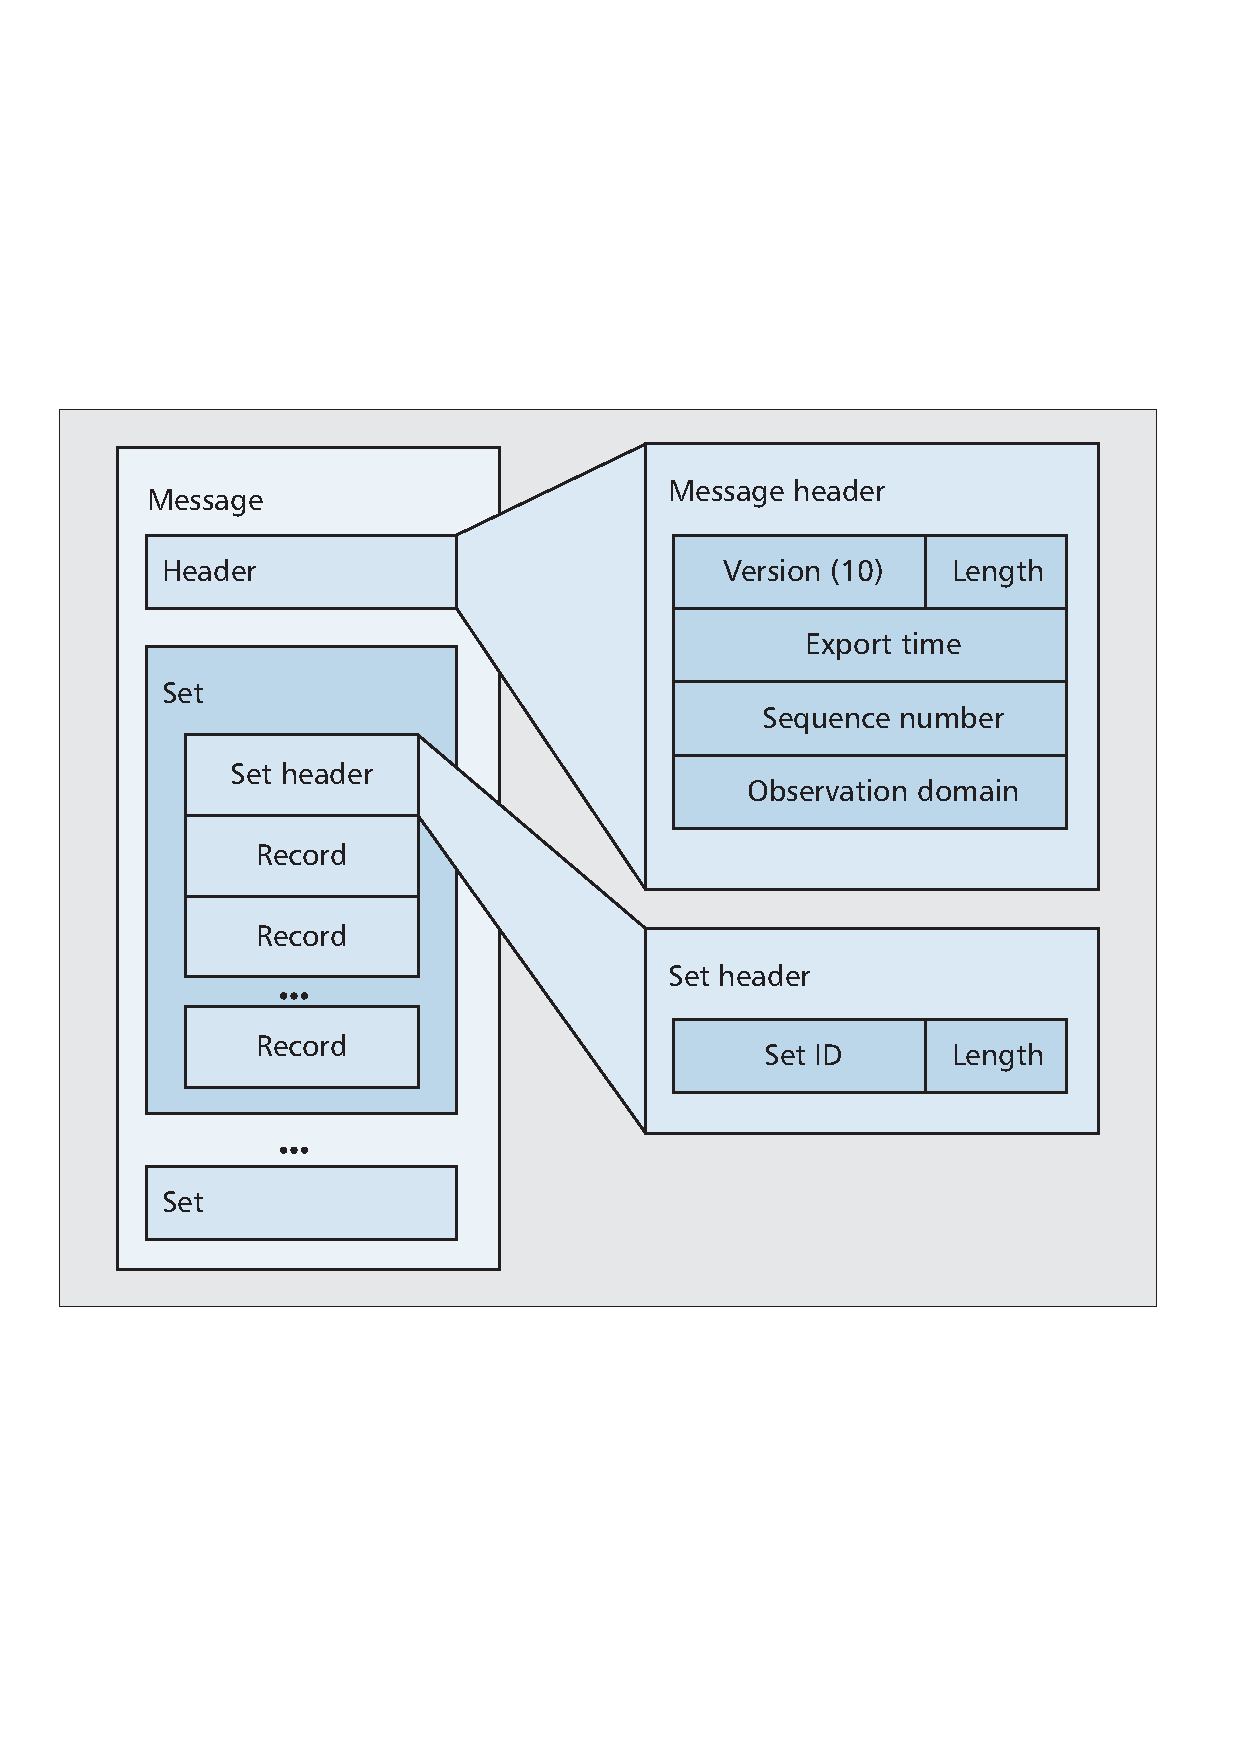
\includegraphics[width=0.7\linewidth]{figures/ipfix-message-structure}
		\caption{IPFIX: Messages \cite{btrammell:2011}}
		\label{fig:ipfix-message-structure}
	\end{minipage}	
	\begin{minipage}[b]{0.49\linewidth}
		\centering
		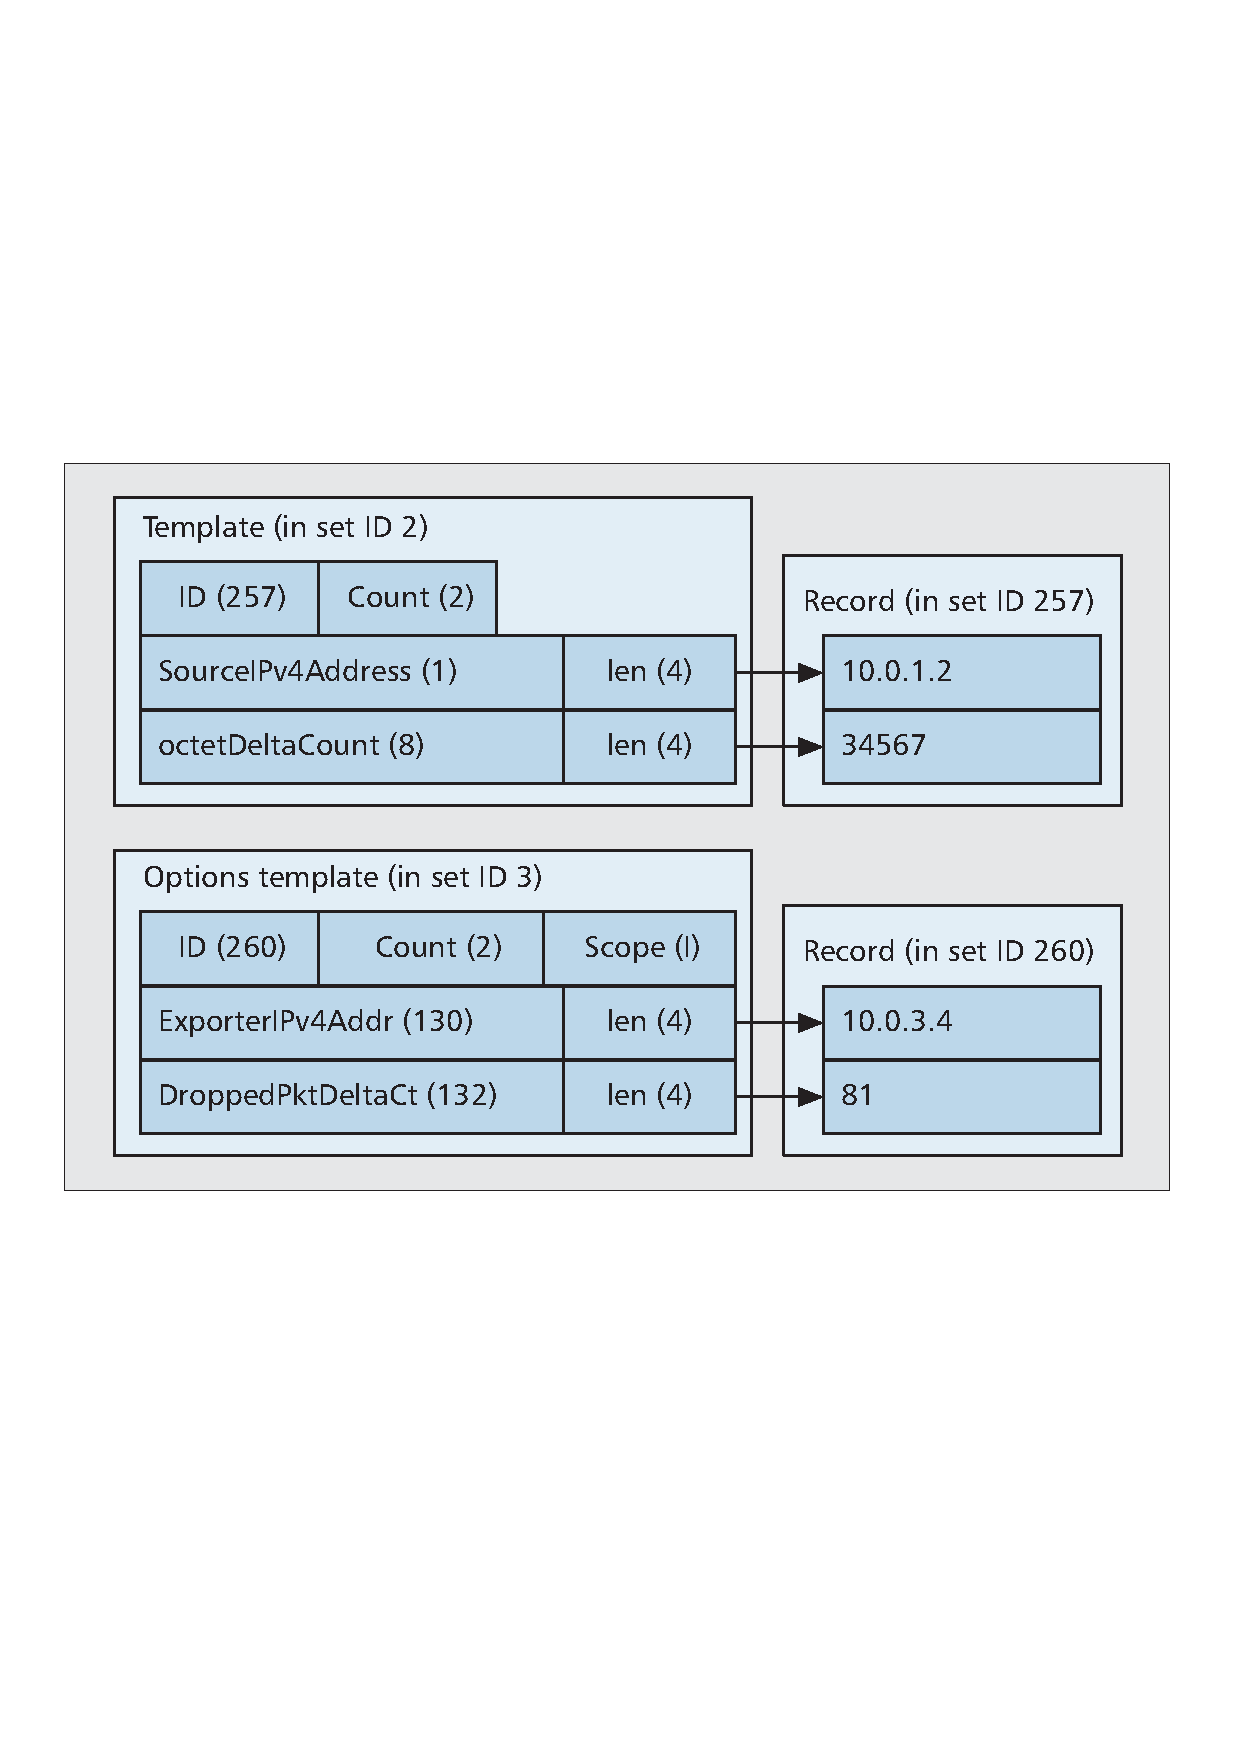
\includegraphics[width=0.7\linewidth]{figures/ipfix-information-element}
		\caption{IPFIX: Templates \cite{btrammell:2011}}
		\label{fig:ipfix-information-element}
	\end{minipage}	
\end{figure}
A message is a fundamental unit of data exchange in \ac{IPFIX}. Each such message consists of a $16$-byte header along with a number of sets as shown in figure $\ref{fig:ipfix-message-structure}$. A set can either be a template or a data set. Each such set in the message again contains a $16$-bit header and a number of records \marginpar{messages and templates} associated with it. Each record within a template set is a template that refers to a data record.  A template consists of a number of \ac{IE}s as shown in figure $\ref{fig:ipfix-information-element}$. These \ac{IE}s are encoded using reduced-length encoding scheme. \ac{IANA} keeps a registry \footnote{\url{http://www.iana.org/assignments/ipfix/ipfix.xml}} of all \ac{IE}s with a $16$-bit ID assigned to them. Templates can also contain enterprise-specific \ac{IE}s that are scoped using \ac{PENs} \footnote{\url{http://www.iana.org/assignments/enterprise-numbers}}. 

\begin{figure}[h!]
\begin{center}
  \includegraphics* [width=0.5\linewidth]{figures/ipfix-transport}	
  \caption{IPFIX: A Transport Session \cite{btrammell:2011}}
  \label{fig:ipfix-transport}
\end{center}
\end{figure}
An \ac{IPFIX} transport session is shown in figure $\ref{fig:ipfix-transport}$. It starts off with the \ac{EP} initiating a connection with the \ac{CP}. Once the connection is established, the \ac{EP} passes on the templates followed by the data that is described by them. These templates can later still be withdrawn by sending a control template of \ac{IE} count zero. The transport session can use either \ac{SCTP}, \ac{TCP} or \ac{UDP} as the \marginpar{transport and security} underlying protocol, although \ac{SCTP} is usually the preferred method given it allows selective reliability and congestion control. \ac{TCP} is supported to allow secure transport over \ac{TLS}, since \ac{DTLS} is only supported over \ac{UDP} and \ac{SCTP}. The connection-less behavior of \ac{UDP} calls for the template retransmission delay and template lifetime parameters to be exchanged between \ac{EP} and \ac{CP}. These transport sessions can also be stored in \ac{IPFIX} files and sent on top application layer protocols. 

A \ac{MIB} to monitor \ac{IPFIX} devices using \ac{SNMP} is defined in \cite{rfc5815}. A similar configuration model to be used by NETCONF and YANG is being worked upon. In addition, several extensions have been defined to expand upon the protocol's functionality. For instance, \cite{rfc5103} defines optional templates to allow \marginpar{management, extensions and future of ipfix} bidirectional flows in a single \ac{IPFIX} export whereas \cite{rfc5474} supports aggregating common properties of multiple flows in a single record. \ac{IPFIX} is even being looked upon as the future application-layer logging protocol as well as the underlying protocol for RESTful architectures. As a result, efforts to support structured data export over \ac{IPFIX} are also under way.

\section{sFlow}\label{sec:sflow}
sFlow \cite{rfc3176} by InMon Corporation is a competing technology used to capture traffic from switches and routers. It consists of an sFlow agent that captures traffic statistics and sends them across to a central data collector, called the sFlow analyzer. In order to be able to accurately monitor traffic at line speeds, the sFlow agent is built on a dedicated ASIC alongside the switching gear. In addition, the captured traffic is sampled before being encapsulated in sFlow datagrams and sent to the analyzer to provide scalability.



\marginpar{sampling mechanisms}
\marginpar{sflow and snmp}
\marginpar{data format}
\marginpar{security considerations}


\todo[inline]{sFlow: Start it! \ldots}
% %***********************************************************
\chapter{Languages and Tools}\label{ch:languages-and-tools}
%***********************************************************

\section{nfdump}\label{sec:nfdump}
\section{flow-tools}\label{sec:flow-tools}
\section{Gigascope}\label{sec:gigascope}

\cleardoublepage
\ctparttext{The semantics and implementation of our in-house flow-record querier has
underwent significant changes in the last few years. This section is dedicated
to perform an inside-out study of the querier, examining all its major (and
minor) changes to allow us to better make a pragmatic stand towards its
overall packaging and improvement. The organization of the section is
described below.

\vspace{50pt}

In chapter $\ref{ch:flowy-design}$ we look into the structure of the flow
query language by discussing each stage of the processing pipeline with their
implementation details. The basic structures of the framework that underpin
the implementation are also discussed. In the end, we ponder over the current
prototype limitation and its suggestive improvements.

In chapter $\ref{ch:flowy-mapreduce}$ we investigate the possibility of making
Flowy Map/Reduce aware. The chapter starts off with a discussion of current
Map/Reduce frameworks and looks into the ways to help parallelize Flowy.

In chapter $\ref{ch:flowy-2}$ and $\ref{ch:f}$ we look into the first attempt
to make Flowy comparable with the state-of-the-art flow-analysis tools. After
drilling down the performance hit sections of the code, we witness how getting
away with PyTables and rewriting the complete core implementation in C helped
make the tool eventually usable. We end by examining the recommended approach
to glue the two implementations together to bring the best of both worlds.

We conclude this discussion in chapter $\ref{ch:flowy-applications}$ by
introducing a number of real-life application scenarios where Flowy has proved
useful. We also looked into a few current bleeding edge research projects
where we believe Flowy could play a vital role in the near future.
}
\part{State of the Art}
%************************************************
\chapter{Flowy}\label{ch:flowy-design}
%************************************************

\section{Processing Pipeline}\label{sec:processing-pipeline}
  \subsection{Splitter}\label{subsec:splitter}
  \subsection{Filter}\label{subsec:filter}
  \subsection{Grouper}\label{subsec:grouper}
  \subsection{Group-Filter}\label{subsec:group-filter}
  \subsection{Merger}\label{subsec:merger}
  \subsection{Ungrouper}\label{subsec:ungrouper}

\section{Python Framework}\label{sec:python-framework}
	\subsection{PyTables and PLY}\label{subsec:pytable-ply}
	\subsection{Records}\label{subsec:records}
	\subsection{Filters and Rules}\label{subsec:filters-rules}
	\subsection{Branches and Branch Masks}\label{subsec:branches-branchmasks}
%***********************************************************************
\chapter{Flowy Improvements using Map/Reduce}\label{ch:flowy-mapreduce}
%***********************************************************************

Flowy, although clearly setting itself apart with its additional functionality to query intricate patterns in the flows demonstrates relatively high execution times when compared to contemporary flow-processing tools. A recent study \cite{pnemeth:thesis:2010} revealed that a sample query run on small record set (around 250MB) took 19 minutes on Flowy as compared to 45 seconds on \texttt{flow-tools}. It, therefore is imperative that the application will benefit from distributed and parallel processing. To this end, recent efforts were made to investigate possibility of making Flowy Map/Reduce aware \cite{pnemeth:thesis:2010}

\section{Map/Reduce Frameworks}\label{sec:map-reduce}
\section{Parallelizing Flowy}\label{sec:parallel-flowy}
	\subsection{Installing Disco}\label{subsec:install-disco}
	\subsection{Slicing Inputs}\label{subsec:slice-input}
		\subsubsection{Using \emph{only} Filters}\label{subsec:filters-only}
		\subsubsection{Using Groupers}\label{subsec:using-groupers}
		\subsubsection{Using Mergers}\label{subsec:using-mergers}
	\subsection{Flowy as a Map Function}\label{subsec:flowy-map}

%**************************************
\chapter{F $(v1)$}\label{ch:flowy-2}
%**************************************

In an attempt to develop a prototype implementation of \ac{NFQL} which will be
comparable with the contemporary flow-record analysis tools, the substitution
of the performance hit sections of the python code was thought out. Flowy
$2.0$ \cite{jschauer:thesis:2011} is the first attempt to try rewriting the
core of the prototype implementation in C.

\section{Flowy Performance Issues}\label{sec:performance-issues}

\begin{table}[h!]
	\begin{tabular}{|c|c|c|c|c|}
	\hline
	no. of records & overall & filter & grouper & merger \\
	\hline
	\hline
	$103k$ & $1177s$ & $28s (2\%)$ & $240s (20\%)$ & $909s (77\%)$\\
	\hline
	$337k$ & $20875s$ & $110s (1\%)$ & $2777s (13\%)$ & $17988s (86\%)$\\
	\hline
	$656k$ & $70035s$ & $202s (0\%)$ & $8499s (12\%)$ & $61334s (87\%)$\\
	\hline
	$868k$ & $131578s$ & $274s (0\%)$ & $15913s (12\%)$ & $115391s (87\%)$\\
	\hline
	$1161k$ & $234714s$ & $1212s (1\%)$ & $25480s (11\%)$ & $208022s (88\%)$\\
	\hline
	\end{tabular}
\caption{Runtime Breakup of Individual Stages \cite{jschauer:thesis:2011}}
\label{tab:flowy2-profiling}
\end{table}

The runtime breakup of individual stages of the processing pipeline as shown
in table \ref{tab:flowy2-profiling} reveal that the grouper and merger incur a
massive performance hit. A quick \marginpar{deep nested loops} investigation
hints towards usage of large deep nested loops in the merger with a worst-case
$O(n^3)$ runtime complexity.

In addition, pushing the flow-records data from one stage of the pipeline to
another involved deep copying of the whole flow data whereby a mere passing
across of a \marginpar{deep copy of flow records} reference across a pipeline
in a branch would have sufficed. Similar behavior is visible when the grouper
when passing group records saved the individual flow-records in a temporary
location tagged with the groups and/or subgroups they belonged to.

The decision to use PyTables to read and write flow-records in
\ac{HDF} format also added to the complexity. Since, the input flow-records
were most of the time \marginpar{pytables and hdf} in either
\texttt{flow-tools} or \texttt{nfdump} file-formats, each time they had to be
converted into \ac{HDF} file formats prior to Flowy's execution which was
unnecessary.


\section{Preliminary Improvements}\label{sec:prelim-improvements}

The python parser written in \ac{PLY} and the validators written for
each stage of the processing pipeline that check for semantics correctness
were left unmodified, since their execution time was invariant of the size of
the input data and slightly varied on the query complexity.

Thread affinity masks were set for each new thread created to delegate the
thread to a separate processor core. \texttt{try/except} blocks were narrowed
down to only code that needed to be exception handled. A test-suite was
developed with few sample queries and input traces to validate Flowy's results
for regression analysis. A \texttt{setup.py} script was written to facilitate
installation of \marginpar{affinity masks, easier installation and
configuration, better profiling and testing, extended command line switches}
Flowy and its dependencies and \texttt{options.py} was replaced with
\texttt{flowy.conf} configuration file with the standard human-readable
key-value pairs. The command line option handling was switched from
\texttt{optparse} to \texttt{argparse} module and a switch was added for easy
profiling. The profiling output was modified as well to allow standard tab
delimiters which can be easily parsed by other tools. The flow query was also
extended to allow file contents to be supplied using \texttt{stdin}. Variable
names that are now part of Python identifiers were renamed.

A custom C library was written to directly read/write data in the
\texttt{flow-tools} format to provide a drop-in replacement for PyTables and
overcome the overhead of format conversions. The library sequentially reads
the complete flow-records into memory to support random access required for
relative filtering. Each flow-record is stored in a \texttt{char} array and
the offsets to each field are stored in a separate \texttt{struct}.
\marginpar{a custom c library to replace pytables, cython to connect the
library to python} The array of such records are indexed allowing fast
retrieval in $O(1)$ time.  The C library was connected to the Python prototype
using Cython \cite{dseljebotn:2009}\cite{wilbers:2009}.  This allowed the
flow-records to be easily referenced by an identifier, thereby giving away the
need to every time copy all the flow-records when moving ahead in the
processing pipeline.  Cython was used since it allowed to write C extensions
in a Pythonic way by strong-typing variables, calling native C libraries and
allowing usage of pointers and structs, thereby providing the best of both
worlds \cite{sbehnel:2011}.


%The current core implementation also strictly adheres to the processing
%pipeline shown in figure \ref{fig:flowy-pipeline}. As such, it is not
%currently possible to skip \marginpar{core limitations} stages. In addition it
%is not currently possible to have more than one merger or grouper in the
%flow-query or aggregate fields in the grouper module since \texttt{char} array
%storage is not possible.



\section{Rule Interfaces}\label{sec:rule-interfaces}


A design decision was made to attempt to rewrite the entire processing
pipeline in C.  However, currently the core can only run absolute filters and
cannot parse the flowquery file. Therefore the execution is triggered by a
tedious manual filling of the \texttt{struct} by the contents of the query.  A
filter \marginpar{filter stage struct} stage \texttt{struct} is shown in
listing \ref{lst:filterrule}. The field to be filtered is indicated using a
\texttt{field\_offset} and \texttt{field\_length} in the \texttt{char} array
of a records. The value to be compared against with is also supplied which can
be either a static value or another field of a record.  \texttt{func} is a
function pointer to the operation that is to be carried out on a record whose
record identifier is passed to it. The filter runs in $O(n)$ time as it needs
to traverse through all the records of the \texttt{char} array.

\lstset{caption=Filter Rule Struct \cite{jschauer:thesis:2011},
				basicstyle=\tiny\ttfamily, tabsize=2, language=C, numbers=left,
        stepnumber=1, numberstyle=\ttfamily\color{gray},
        keywordstyle=\color{blue}, frame=shadowbox, rulesepcolor=\color{black},
			  label=lst:filterrule, aboveskip=20pt, captionpos=b}
\begin{lstlisting}
struct filter_rule {
	size_t field_offset;
	uint64_t value;
	uint64_t delta;
	bool (*func)(
		char *record,
		size_t field_offset,
		uint64_t value,
		uint64_t delta);
};
\end{lstlisting}


\section{Efficient Rule Processing}\label{sec:efficient-rule-processing}

The comparison operations, previously were required to make costly checks on
the length of the field type passed to them, to be able to make appropriate
casts. Such checks are now no longer needed. F $(v1)$ now allows filtering of
records via two methods: using specialized comparison functions or using one
main fall through \texttt{switch} statement. The implementation defaults to
using specialized comparison functions to encourage modularity in source code.

\lstset{caption=Auto Generated Comparison Functions \cite{jschauer:2012},
				tabsize=2, language=C, numbers=left,stepnumber=1,
				numberstyle=\ttfamily\color{gray}, keywordstyle=\color{blue},
				frame=shadowbox, rulesepcolor=\color{black},
			  label=lst:autocompfunc, aboveskip=20pt, captionpos=b}
\begin{lstlisting}
bool filter_eq_uint8_t(...);
bool filter_eq_uint16_t(...);
...
\end{lstlisting}

In the default method, there is a comparison function defined for every
possible field length $(33)$ and comparison operations $(19)$. These functions
are generated using a Python script
\footnote{\texttt{scripts/generate-functions.py}} and are declared/defined in
\texttt{auto\_comps.\{h,c\}} as shown in listing $\ref{lst:autocompfunc}$. The
rule definitions are now able to make calls \marginpar{using function pointers
and switch cases} using a function name derived from the combination of field
length, delta type and operation. This subverts the need to define complex
branching statements and reduces complexity. In the other method, the logic is
executed by comparing the field length and the operation by falling through a
huge switch statement.  Such a huge switch statement is again generated using
the same Python script and is defined in \texttt{auto\_switch.c} as shown in
listing $\ref{lst:autoswitch}$.


\lstset{caption=Auto Generated Switch Statement \cite{jschauer:2012},
				tabsize=2, language=C, numbers=left,stepnumber=1,
				numberstyle=\ttfamily\color{gray}, keywordstyle=\color{blue},
				frame=shadowbox, rulesepcolor=\color{black},
			  label=lst:autoswitch, aboveskip=20pt, captionpos=b}
\begin{lstlisting}
switch (group_modules[k].op) {
  case RULE_EQ | RULE_S1_8 | RULE_S2_8 | RULE_ABS:
  case RULE_EQ | RULE_S1_8 | RULE_S2_8 | RULE_REL:
  ...
\end{lstlisting}





\section{Faster Grouping Approach}\label{sec:faster-grouper}
A typical grouper module is shown listing \ref{lst:fv2-grouper-module}. In
order to be able to make comparisons on field offsets, the grouper initially
creates a copy of the pointers in the filtered recordset. A n\"aive approach
is to linearly walk through \marginpar{possible grouping approaches} all the
pointers against each pointer in the copy leading to a complexity of $O(n^2)$.
A smarter approach is to put the copy in a hash table and then try to map each
pointer while walking down the recordset once, leading to a complexity of
$O(n)$. The hash table approach, although will work on this specific example,
will fail badly on other relative comparisons.

\lstset{caption=A Grouper Module,
				tabsize=2, language=bash, numbers=left,stepnumber=1,
        basicstyle=\tiny\ttfamily, numberstyle=\ttfamily\color{gray},
        keywordstyle=\color{blue}, frame=shadowbox,
        rulesepcolor=\color{black}, label=lst:fv2-grouper-module,
        aboveskip=20pt, captionpos=b}
\begin{lstlisting}
grouper g1 {
  srcIP = srcIP
  dstIP = dstIP
}
\end{lstlisting}

It is clear that a middle ground compromise was needed. As a result, using a
binary search after a quick sort on the filtered recordset was thought out. To
achieve this, the array of pointers to the copy are sorted according to the
offset on the right side of the comparsion of the first grouping rule.
\marginpar{using quick sort and binary search} Such a sorted array of pointers
is then traversed linearly to find unique values. This helps the grouper
perform binary searches to find records that will eventually group together.
The preprocessing step takes $O(n*lg(n)) + O(n)$ in the worst case, with a
$O(n*lg(k))$ for binary search on the entire recordset. The implementation of
this idea is currently broken and segfaults at multiple stages. In essence,
this approach is not currently used in practise and quite some effort is
needed to bring it to life.


\section{Benchmarks}\label{sec:benchmarks}

\begin{table}[h!]
	\begin{center}
		\begin{tabular}{|c|c|c|}
		\hline
		Number of records & Flowy & F $(v1)$ \\
		\hline
		\hline
		$103k$ & $1177s$ & $0.3s$\\
		\hline
		$337k$ & $20875s$ & $3.4s$\\
		\hline
		$656k$ & $70035s$ & $13s$\\
		\hline
		$868k$ & $131578s$ & $23s$\\
		\hline
		$1161k$ & $234714s$ & $86s$\\
		\hline
		\end{tabular}
	\end{center}
\caption{Flowy vs $F (v1)$ \cite{jschauer:thesis:2011}}
\label{tab:flowy2-benchmarks}
\end{table}

The benchmarks in table \ref{tab:flowy2-benchmarks} show the relative
comparison of Flowy \cite{kkanev:thesis:2009} with F $(v1)$
\cite{jschauer:thesis:2011}. As the author appropriately points out, an
accurate comparison of Flowy with F $v1$ cannot be done accurately, since, the
the C execution engine \marginpar{vs flowy} lacks many feature-set and
pipeline stages. However, running a common flow query that can be run on both
the implementations was used and it was not surprising that F $(v1)$ was in
orders of magnitude faster in comparison.

\lstset{caption=F$(v1)$ vs {\texttt{flow-tools, nfdump}} \cite{jschauer:2012},
				tabsize=2, language=C, numbers=left,stepnumber=1,
				numberstyle=\ttfamily\color{gray}, keywordstyle=\color{blue},
				frame=shadowbox, rulesepcolor=\color{black},
			  label=lst:f-benchmark-queries, aboveskip=20pt, captionpos=b}
\begin{lstlisting}
src port 80
src port 80 or dst port 25
src port 443 or (src port 80 and dst port 25)
\end{lstlisting}

In order to evaluate how well F now performs with these added improvements,
the authors decided to compare it with the state-of-the-art flow-processing
tools: \marginpar{vs flow-tools and nfdump} \texttt{flow-tools}
\cite{sromig:2000} and \texttt{nfdump} \cite{phaag:2006}. A set of $3$ queries
involving only absolute filters was defined as shown in listing
$\ref{lst:f-benchmark-queries}$ and evaluated on a set of $500K-10M$
flow-records. It turned out that F $(v1)$ performed as well if not better than
the other flow tools.

%**************************************
\chapter{F}\label{ch:f}
%**************************************

In lieu of the significant leaps made by Flowy $2.0$ in making the initial prototype usable, additional efforts were made by the same author to work upon the enlisted areas of improvements mentioned in $\ref{sec:flowy2-future}$. To mark this evolution of initial prototype to the current bleeding edge state, it was decided to rename the implementation to F \cite{jschauer:2012} with an exhaustive performance evaluation against the state-of-the-art flow processing tools \cite{sromig:2000, phaag:2006} that operate on absolute filters.

\section{Rule Interfaces}\label{sec:rule-interfaces}
The design of the rule interfaces for a flow-query was rethought. An object-oriented approach was followed to abstract out details into multiple levels of inheritance. The \texttt{flowquery} struct for instance, is the parent of all the rule interfaces as shown in listing $\ref{lst:flowqueryrule}$.
\lstset{caption=Flow Query Struct \cite{jschauer:2012}, 
				tabsize=2, language=C, numbers=left,stepnumber=1,
				numberstyle=\ttfamily\color{gray}, keywordstyle=\color{blue},
				frame=shadowbox, rulesepcolor=\color{black}, 	
			  label=lst:flowqueryrule, aboveskip=20pt, captionpos=b}
\begin{lstlisting}
struct flowquery {
	size_t num_branches;
	struct branch_info *branches;
	struct merger_rule **mrules;
};
\end{lstlisting}

\texttt{branch\_info} struct defines rules for each branch. It conglomerates filter, grouper and group-filter stages as shown in listing $\ref{lst:branchinforule}$. 
\lstset{caption=Branch Info Struct \cite{jschauer:2012}, 
				tabsize=2, language=C, numbers=left,stepnumber=1,
				numberstyle=\ttfamily\color{gray}, keywordstyle=\color{blue},
				frame=shadowbox, rulesepcolor=\color{black}, 	
			  label=lst:branchinforule, aboveskip=20pt, captionpos=b}
\begin{lstlisting}
struct branch_info {
	int branch_id;
	struct ft_data *data;
	struct filter_rule *filter_rules;
	size_t num_filter_rules;
	struct grouper_rule *group_modules;
	size_t num_group_modules;
	struct grouper_aggr *aggr;
	size_t num_aggr;
	struct gfilter_rule *gfilter_rules;
	size_t num_gfilter_rules;
	struct group **filtered_groups;
	size_t num_filtered_groups;
};
\end{lstlisting}

\begin{center}
\begin{minipage}{.44\textwidth}
	\lstset{caption=Grouper Struct \cite{vperelman:thesis:2010}, 
					tabsize=2, language=C, numbers=left,stepnumber=1,
					basicstyle=\tiny\ttfamily,numberstyle=\ttfamily\color{gray},
					keywordstyle=\color{blue},frame=shadowbox, rulesepcolor=\color{black}, 	
				  label=lst:grouperrule, aboveskip=20pt, captionpos=b}
	\begin{lstlisting}
	struct grouper_rule {
		size_t field_offset1;
		size_t field_offset2;
		uint64_t delta;
		uint16_t op;
		bool (*func)(
		  struct group *group,
		  size_t field_offset1,
		  char *record2,
		  size_t field_offset2,
		  uint64_t delta);
	};
	\end{lstlisting}
\end{minipage}
\hfill
\begin{minipage}{.44\textwidth}
	\lstset{caption=Group Struct \cite{vperelman:thesis:2010}, 
					tabsize=2, language=C, numbers=left,stepnumber=1,
					basicstyle=\tiny\ttfamily, numberstyle=\ttfamily\color{gray},
					keywordstyle=\color{blue},frame=shadowbox, rulesepcolor=\color{black}, 	
				  label=lst:grouprule, aboveskip=20pt, captionpos=b}
	\begin{lstlisting}
	struct group {
		char        **members;
		size_t      num_members;
		struct aggr *aggr;
		uint32_t    start;
		uint32_t    end;
	};

	struct aggr {
	  size_t   num_values;
	  uint64_t *values;
	};
	\end{lstlisting}
\end{minipage}
\end{center}
The group-filter struct is similar to the filter struct previously shown in listing $\ref{lst:filterrule}$. The grouper struct is shown in listing $\ref{lst:grouperrule}$ and is used to perform relative comparison on the flow-records. It takes in offsets of the fields to be grouped, their lengths and a comparison function. Possible comparison functions are \texttt{eq}, \texttt{ne}, \texttt{lt}, \texttt{gt}, \texttt{le} and \texttt{ge}. The comparison function creates a \texttt{group} instance, a pointer to which is passed to it. The group struct is shown in listing $\ref{lst:grouprule}$ which apart from the information about the members, also points to a grouper aggregation struct that contains meta-information resulting from calling an aggregation function. 
\lstset{caption=Grouper Aggregation Struct \cite{jschauer:2012}, 
				tabsize=2, language=C, numbers=left,stepnumber=1,
				numberstyle=\ttfamily\color{gray}, keywordstyle=\color{blue},
				frame=shadowbox, rulesepcolor=\color{black}, 	
			  label=lst:grouperaggrrule, aboveskip=20pt, captionpos=b}
\begin{lstlisting}
struct grouper_aggr {
	int module;
	size_t field_offset;
	struct aggr (*func)(
	  char **group_records,
	  size_t num_records,
	  size_t field_offset);
};
\end{lstlisting}
The grouper aggregation struct is shown in listing $\ref{lst:grouperaggrrule}$ and consists of the module to aggregate over, the field offset and the aggregation function. Possible aggregation functions are \texttt{static}, \texttt{count}, \texttt{union}, \texttt{min/max}, \texttt{mean/median}, \texttt{stddev}, \texttt{sum/prod}, \texttt{and/or/xor}. The merger stage struct is the same as was previously shown in listing $\ref{lst:mergerrrule}$ and allows relative comparison between groups from different branches. 

The rules are now possible to be written in \ac{CNF}. \ac{CNF} allow the flexibility to define every possible logical expression with the available comparison operations. The comparison (\texttt{>>} and \texttt{<<}) and the \texttt{intersect} aggregation operations still need to be implemented though as was previously mentioned in section $\ref{subsec:additional-functionality}$. 

\section{Flowy $2.0$ Improvements}\label{sec:flowy-2-improvements}
This study focusses on optimizing deep nested loops in each processing stage and improving the overall complexity of the grouper and merger as previous enlisted in sections $\ref{subsec:special-fns}$ and $\ref{subsec:search-trees}$.

\subsection{Efficient Rule Processing}\label{sec:rule-processing}
The comparison operations, previously were required to make costly checks on the length of the field type passed to them, to be able to make appropriate casts. Such checks are now no longer needed. F now allows filtering of records (and groups) via two methods: using specialized comparison functions or using one main fall through \texttt{switch} statement. The implementation defaults to using specialized comparison functions to encourage modularity in source code. 

\lstset{caption=Auto Generated Comparison Functions \cite{jschauer:2012}, 
				tabsize=2, language=C, numbers=left,stepnumber=1,
				numberstyle=\ttfamily\color{gray}, keywordstyle=\color{blue},
				frame=shadowbox, rulesepcolor=\color{black}, 	
			  label=lst:autocompfunc, aboveskip=20pt, captionpos=b}
\begin{lstlisting}
bool filter_eq_uint8_t(...);
bool filter_eq_uint16_t(...);
...
\end{lstlisting}
In the default method, there is a comparison function defined for every possible field length $(33)$ and comparison operations $(19)$. These functions are generated using a \marginpar{using function pointers}Python script \footnote{\texttt{fun\_gen.py}} and are declared/defined in \texttt{auto\_comps.\{h,c\}} as shown in listing $\ref{lst:autocompfunc}$. The rule definitions are now able to make calls using a function name derived from the combination of field length, delta type and operation. This subverts the need to define complex branching statements and reduces complexity. 

\lstset{caption=Auto Generated Switch Statement \cite{jschauer:2012}, 
				tabsize=2, language=C, numbers=left,stepnumber=1,
				numberstyle=\ttfamily\color{gray}, keywordstyle=\color{blue},
				frame=shadowbox, rulesepcolor=\color{black}, 	
			  label=lst:autoswitch, aboveskip=20pt, captionpos=b}
\begin{lstlisting}
switch (group_modules[k].op) {
  case RULE_EQ | RULE_S1_8 | RULE_S2_8 | RULE_ABS:
  case RULE_EQ | RULE_S1_8 | RULE_S2_8 | RULE_REL:
  ...
\end{lstlisting}
In the other method, the logic is executed by comparing the field length and the operation \marginpar{using switch statement} by falling through a huge switch statement. Such a huge switch statement is again generated using the same Python script and is defined in \texttt{auto\_switch.c} as shown in listing $\ref{lst:autoswitch}$.  

\subsection{Binary Search for
 						Fast Relative Comparisons}\label{sec:binary-search}
\section{Benchmarks}\label{sec:f-benchmarks}
%***********************************************************
\chapter{NFQL: Applications}\label{ch:flowy-applications}
%***********************************************************

\ac{NFQL} helped to underpin a number of recent research efforts to solve
real-world application problems that were deemed difficult before. This was
possible due to the power and flexibility of the flow-query language to suit
itself from generic to specific needs thereby opening doors of innovation.
This section documents such efforts that use the in-house flow query language
as well as a few others that exploit the flow level characteristics of the
traffic patterns in general.

\section{Application Identification using Flow
Signatures}\label{sec:application-signatures}
The idea behind this study was to identify applications using flow traces on a network by analyzing potential left-behind signatures that describe them \cite{vperelman:2011, vperelman:thesis:2010}. This was based on the hypothesis that each application type generates unique flow signatures that might work as a fingerprint feature. To achieve this, a collection of network traces were recorded from several users and subsequently analyzed. The identified signatures were formalized by writing flow queries that were executed on Flowy \cite{kkanev:2010}. Several separate instances of the network traces were queried to evaluate the approach and come to a conclusion.

\lstset{caption=Skype Application Signature \cite{vperelman:thesis:2010},
				tabsize=2, language=C, numbers=left,stepnumber=1,
				basicstyle=\tiny\ttfamily, numberstyle=\ttfamily\color{gray},
				keywordstyle=\color{blue}, frame=shadowbox, rulesepcolor=\color{black},
			  label=lst:skypequery, aboveskip=20pt, captionpos=b}
\begin{lstlisting}
splitter S {}

...

merger M {
	module m1 {
		branches A, B
		A.srcip = B.srcip
		A o B OR B o A
	}
	export m1
}

ungrouper U {}

"input" -> S
S branch A -> F_SSDP -> G_SSDP -> GF_SSDP -> M
S branch B -> F_NAT_PMP -> G_NAT_PMP -> GF_NAT_PMP -> M
M -> U -> "output"
\end{lstlisting}
A formalized Flowy query to identify Skype from the flow traces for an instance is described in listing \ref{lst:skypequery}. The filter, grouper and group-filter sections of each branch are shown separately in listings \ref{lst:skypebranchA} and \ref{lst:skypebranchB}. Additional queries identifying variety of web browsers, mail clients, IM clients and media players can be found in \cite{vperelman:thesis:2010}.

\begin{center}
\begin{minipage}{.44\textwidth}
	\lstset{caption=Branch A \cite{vperelman:thesis:2010},
					tabsize=2, language=C, numbers=left,stepnumber=1,
					basicstyle=\tiny\ttfamily,numberstyle=\ttfamily\color{gray},
					keywordstyle=\color{blue},frame=shadowbox, rulesepcolor=\color{black},
				  label=lst:skypebranchB, aboveskip=20pt, captionpos=b}
	\begin{lstlisting}
	filter F_SSDP {
		dstport = 1900
		port = protocol("UDP")
		dstip = 239.255.255.250
	}

	grouper G_SSDP {
		module g1 {
			srcip = scrip
			dstip = dstip
			srcport = srcport
		}
		aggregate srcip, sum(bytes) as B
	}

	groupfilter GF_SSDP {
		B = 321
	}
	\end{lstlisting}
\end{minipage}
\hfill
\begin{minipage}{.44\textwidth}
	\lstset{caption=Branch B \cite{vperelman:thesis:2010},
					tabsize=2, language=C, numbers=left,stepnumber=1,
					basicstyle=\tiny\ttfamily, numberstyle=\ttfamily\color{gray},
					keywordstyle=\color{blue},frame=shadowbox, rulesepcolor=\color{black},
				  label=lst:skypebranchA, aboveskip=20pt, captionpos=b}
	\begin{lstlisting}
	filter F_NAT_PMP {
		dstport = 5351
		port = protocol("UDP")
	}

	grouper G_NAT_PMP {
		module g1 {
			srcip = scrip
			dstip = dstip
		}
		aggregate srcip, sum(bytes) as B
	}

	groupfilter GF_NAT_PMP {
		B = 160
	}
	\end{lstlisting}
\end{minipage}
\end{center}
The filter \texttt{F\_SSDP} is used to identify the four identical \ac{UDP} multicast messages the client sends out using \ac{SSDP} \cite{mbodlaender:2005}. Similarly \texttt{F\_NAT\_PMP} filter is used to identify four \ac{NAT-PMP} \cite{draft-cheshire-nat-pmp-03} messages sent over UDP. The groupers \texttt{G\_SSDP} and \texttt{G\_NAT\_PMP} group together flow records \marginpar{skype application signature} with the same source and destination IP address and the aggregate clauses describe the meta information with unique source IP addresses for each group records along with the total bytes carried within each group. The meta information is used to further filter the group-records in \texttt{GF\_SSDP} and \texttt{GF\_NAT\_PMP} modules.

\begin{table}[h!]
	\begin{center}
		\tiny
		\begin{tabular}{|c|c|c|c|c|c|}
		\hline
		UserID & Skype & Opera & Amarok & Chrome & Live \\
		\hline
		\hline
		u$0$ & \ding{52} & \ding{109} & \ding{54} & \ding{109} & \ding{109} \\
		\hline
		u$1$ & \ding{52} & \ding{109} & \ding{109} & \ding{109} & \ding{109} \\
		\hline
		u$2$ & \ding{109} & \ding{109} & \ding{109} & \ding{109} & \ding{109} \\
		\hline
		u$3$ & \ding{52} & \ding{109} & \ding{54} & \ding{109} & \ding{109} \\
		\hline
		u$4$ & \ding{109} & \ding{109} & \ding{109} & \ding{109} & \ding{109} \\
		\hline
		u$5$ & \ding{52} & \ding{109} & \ding{52} & \ding{52} & \ding{109} \\
		\hline
		u$6$ & \ding{109} & \ding{109} & \ding{109} & \ding{109} & \ding{109} \\
		\hline
		u$7$ & \ding{109} & \ding{52} & \ding{52} & \ding{109} & \ding{109} \\
		\hline
		u$8$ & \ding{109} & \ding{109} & \ding{109} & \ding{109} & \ding{109} \\
		\hline
		u$9$ & \ding{52} & \ding{52} & \ding{52} & \ding{52} & \ding{109} \\
		\hline
		\end{tabular}
	\end{center}
\caption{Application Flow Signatures: Results \cite{vperelman:thesis:2010}}
\label{tab:flow-sig-results}
\end{table}
The identification results obtained from the analysis of flow-traces from ten unique users are compiled together in table \ref{tab:flow-sig-results}. The results demonstrate a success rate of $96\%$ for the five applications tested.  This study reveals that it is possible to identify applications from their network flow fingerprints and is \marginpar{success rate} a first step towards automating the complete process whereby machine learning techniques would be used to automatically generate flow-queries and identify new applications and even more so newer versions of the same application.

\section{Cybermetrics: User Identification}\label{sec:cybermetrics}

The idea of identification of users based on biometric patterns such as keystroke dynamics \cite{fbergadano:2002}, mouse interactions \cite{aahmed:2007} or activity cycles in online games \cite{kchen:2007} has been long known. This study takes the idea even further by using flow-record patterns as a characteristic (cybermetrics) to identify a user on a network \cite{nmelnikov:thesis:2010, nmelnikov:2010}. Such a cybermetric user identification can be used for the purpose of providing secure access, system administration and network management. The feature extraction module of the analyzer as shown in figure \ref{fig:cybermetrics-overview} uses three distinct feature sets that could possibly be used to identify a user from a flow-record trace.
\begin{figure}[h!]
\begin{center}
  \includegraphics* [width=0.7\linewidth]{figures/cybermetrics-overview}
  \caption{Cybermetrics: Overview \cite{nmelnikov:thesis:2010}}
  \label{fig:cybermetrics-overview}
\end{center}
\end{figure}

Initial research efforts started with identifying application signatures in flow-records in \cite{vperelman:2011, vperelman:thesis:2010} and became relevant because different people have different preferences in the applications they use \marginpar{application signatures} and as such a set of applications in flow-records is a characteristic feature of a user. Flowy queries were formalized for four different set of applications and tested against a known set of users. The evaluation results of the derived queries as shown in table \ref{tab:flow-sig-results} demonstrated a strong evidence of presence (or absence) of applications and thereby provided an eventual marker for user identification.

\begin{figure}[h!]
\begin{center}
  \includegraphics* [width=0.60\linewidth]{figures/cybermetrics-geography}
  \caption{Geographical Preferences \cite{nmelnikov:thesis:2010}}
  \label{fig:cybermetrics-geography}
\end{center}
\end{figure}
The authors also looked into the geographical affiliations of different users by analyzing the \ac{ccTLD} of the browsed websites. They proposed a hypothesis that a user's origins strongly \marginpar{geographical preferences} influences their browsing activity. The analysis of the results established that the top five visited \ac{ccTLD}s constituted more than $85\%$ of the overall number of a user's visits as shown in figure \ref{fig:cybermetrics-geography}.

\begin{figure}[h!]
\begin{center}
  \includegraphics* [width=0.6\linewidth]{figures/cybermetrics-daily-distrib}
  \caption{Daily Distributions for HTTP Traffic \cite{nmelnikov:thesis:2010}}
  \label{fig:cybermetrics-daily-distrib}
\end{center}
\end{figure}
In the end, the authors introduced a proof-of-concept method of user differentiation based on statistical features. These features considered daily distributions of parameters that were based on different port numbers. \marginpar{flow-record statistics}For instance, figure \ref{fig:cybermetrics-daily-distrib} shows the daily distribution of different users based on their \ac{HTTP} traffic usage. It was also witnessed that the time duration also played a key role in the process of feature formation, whereby the number of longer flows increased with the duration and consequently resulted in higher cross-correlations as shown in figure \ref{fig:cybermetrics-cross-correlate}
\begin{figure}[h!]
\begin{center}
  \includegraphics* [width=0.6\linewidth]{figures/cybermetrics-cross-correlate}
  \caption{Cross Correlation of Traces
					 \cite{nmelnikov:thesis:2010}}
  \label{fig:cybermetrics-cross-correlate}
\end{center}
\end{figure}

This research is a first attempt to identify users based on their network flow fingerprints and the on-going effort is focussing on sophisticated machine learning techniques to learn behavioral patterns of known users to identify them in the future from their current network-flow traces.

\section{IPv$6$ Transition Failure Identification}\label{sec:ipv6transeval}
The IPv$4$ address space depletion is upon us and has become more imminent in the last few years. While IPv$6$ can readily expand the extent of the Internet, deploying it alone is clearly not a solution today and hence there are a continuum of transitioning solutions that would help in this migration. In this study \cite{vbajpai:2012} we evaluated the compatibility of popular applications with such transitioning solutions: NAT$64$ \cite{rfc6146} and Dual-Stack Lite \cite{rfc6333}. The goal was to find potential failures by identifying application failure signatures left behind in the flow-record traces using Flowy. These failure signatures could later be used by service providers to automate the detection and eventually shorten the deployment verification cycle.

\begin{figure}[h!]
\begin{center}
  \includegraphics* [width=0.8\linewidth]{figures/ipv6transeval-nat64-setup}
  \caption{NAT$64$ Setup \cite{vbajpai:2012}}
  \label{fig:ipv6transeval-nat64-setup}
\end{center}
\end{figure}
In the NAT$64$ deployment testbed as shown in figure \ref{fig:ipv6transeval-nat64-setup}, the authors witnessed failure in $3$ applications: Skype, OpenVPN and Transmission. Flowy queries were defined to \marginpar{application operation under NAT$64$} establish failure signatures for each application. A formalized Flowy query to identify Skype failure signature for an instance is described in listing \ref{lst:skypefailure}. The filter sections of each branch are shown separately in listings \ref{lst:skypefailurebranchA} and \ref{lst:skypefailurebranchB}.
\begin{center}
\begin{minipage}{.44\textwidth}
	\lstset{caption=Branch A \cite{vbajpai:2012},
					tabsize=2, language=C, numbers=left,stepnumber=1,
					basicstyle=\tiny\ttfamily,numberstyle=\ttfamily\color{gray},
					keywordstyle=\color{blue},frame=shadowbox, rulesepcolor=\color{black},
				  label=lst:skypefailurebranchA, aboveskip=20pt, captionpos=b}
	\begin{lstlisting}
	filter f-mDNS {
	  dstport = 5353
	  srcport = 5353
	  dstip = 224.0.0.251
	  duration > 1 sec
	  duration < 5 sec
	}
	\end{lstlisting}
\end{minipage}
\hfill
\begin{minipage}{.44\textwidth}
	\lstset{caption=Branch B-C-D \cite{vbajpai:2012},
					tabsize=2, language=C, numbers=left,stepnumber=1,
					basicstyle=\tiny\ttfamily, numberstyle=\ttfamily\color{gray},
					keywordstyle=\color{blue},frame=shadowbox, rulesepcolor=\color{black},
				  label=lst:skypefailurebranchB, aboveskip=20pt, captionpos=b}
	\begin{lstlisting}
	filter f-login1 {
	  dstport = 443
	  duration > 55 sec
	  duration < 59 sec
	}
	\end{lstlisting}
\end{minipage}
\end{center}

Filter \texttt{f-mDNS} is used to filter multicast messages used by Skype to discover clients in the link-local network sent to the destination IP address-port combination $(224.0.0.251:5353)$. Filter \texttt{f-login1} is used to filter $3$ unsuccessful attempts to contact the login server each in a separate branch. The \marginpar{skype failure signature} source port and the duration increases with decreasing number of packets for each subsequent flow.
\lstset{caption=Skype Failure Signature \cite{vbajpai:2012},
				tabsize=2, language=C, numbers=left,stepnumber=1,
				basicstyle=\tiny\ttfamily, numberstyle=\ttfamily\color{gray},
				keywordstyle=\color{blue}, frame=shadowbox, rulesepcolor=\color{black},
			  label=lst:skypefailure, aboveskip=20pt, captionpos=b}
\begin{lstlisting}
splitter S {}

...

grouper g-login1 {
  module g1 {
    srcport = srcport
    dstip = dstip
    dstport = dstport
  }
  aggregate srcip, dstip, srcport, td,
  sum(packets) as pckt-sum, count(rec_id) as n
}

merger M {
  branches mDNS, LOGIN1, LOGIN2, LOGIN3

  LOGIN1.srcip = LOGIN2.srcip
  LOGIN2.srcip = LOGIN3.srcip
  LOGIN1.dstip = LOGIN2.dstip
  LOGIN2.dstip = LOGIN3.dstip

  LOGIN1.srcport = LOGIN2.srcport rdelta 1
  LOGIN2.srcport = LOGIN3.srcport rdelta 1

  LOGIN1.pckt-sum > LOGIN2.pckt-sum
  LOGIN2.pckt-sum > LOGIN3.pckt-sum

  mDNS.td < LOGIN1.td
  mDNS.td < LOGIN2.td
  mDNS.td < LOGIN3.td

  mDNS < LOGIN1
  mDNS < LOGIN2
  mDNS < LOGIN3
}

"input"-> S
S br mDNS -> f-mDNS -> g-mDNS -> gf-mDNS -> M
S br LOGIN1 -> f-login1 -> g-login1 -> gf-login1 -> M
S br LOGIN2 -> f-login2 -> g-login2 -> gf-login2 -> M
S br LOGIN3 -> f-login3 -> g-login3 -> gf-login3 -> M
M -> U -> "output"

\end{lstlisting}
The groupers count the number of packets in each flow-records using \texttt{pckt-sum} which is later utilized by the merger stage to distinguish the branches. The group-filter stage finally is used to filter out groups with more than one record.

The NAT$64$ translation works when the applications running on the IPv$6$-only host explicitly make DNS requests to allow DNS$64$ to capture and masquerade them as fake IPv$6$ addresses that are eventually \marginpar{failure when using IPv$4$ literals}sent to the NAT$64$ box. If the applications use IPv$4$ literals to contact the servers, DNS$64$ is skipped and therefore NAT$64$ cannot perform the translation. This was reason behind the failure of the other two applications (OpenVPN and Transmission).

This study sets across a baseline to automate the failure detection by formalizing queries against flow-records. While a more exhaustive study encompassing wider set of applications still needs to be carried out, it is imperative that this unique approach is not just limited to IPv$6$ transition technologies, but can be utilized to identify failures in more generic cases.

\section{OpenFlow}\label{sec:openflow}
OpenFlow \cite{nmckeown:2008} is an open standards protocol that runs between an Ethernet switch and an OpenFlow controller (a software designed to run on a x$86$ server) to securely manage the forwarding plane of the switch over the network as shown in figure \ref{fig:openflow-architecture}. This enables the controller to push out policies that dictate how to process flow-records crossing the networking infrastructure to eventually improve bandwidth, reduce latency and save power.
\begin{figure}[h!]
\begin{center}
  \includegraphics* [width=0.5\linewidth]{figures/openflow}
  \caption{OpenFlow Architecture \cite{newscientist:2009}}
  \label{fig:openflow-architecture}
\end{center}
\end{figure}

OpenFlow initially started as a way to allow researchers to experiment with new ideas in sufficiently realistic settings by allowing the live production networking gear to open a narrow programmable external interface to it whereby at the same time keeping the inner workings of the gear hidden and proprietary.  The idea took off outside the \marginpar{motivation} academic setting in recent years with the need of data centers requiring to run large-scale map/reduce jobs with full cross-sectional bandwidth. Such a requirement called for flexible forwarding and programmable networks to meet the application-specific needs. Today, the commercial underpinning of OpenFlow are driven by the \ac{IaaS} providers trying to virtualize their network architecture to solve the issue of multi-tenancy to implement \ac{NaaS} architectures \cite{tbenson:2011}.

An OpenFlow switch manages a flow table to keep record of the flows crossing it. A flow table contains a packet header, an action and some statistical information about the flow. OpenFlow defines a common set of methods to program such \marginpar{programming flows} flow tables irrespective of the way different vendors internally defined them. This allows a network administrator to partition the incoming traffic into numerous \ac{vLANs} thereby isolating the production and several experimental networks at the layer 2 level. Now, with the a complete suite of OpenFlow software stack defined on top of the controller, such a power is also available at the hands of the developers that gives them the ability to control the flow tables themselves and even decide the routes for their flow.

The OpenFlow protocol in itself is like an x$86$ instruction-set by itself. However, there is a lot of innovation possible at the software stack layer that can be built on top the controller that exposes the API and pushes this low-level instruction-set to the networking gear. For instance, the stack can deploy \marginpar{software stack} network-wide policies and administer \ac{ACLs} for each incoming flow or  allow seamless handover of mobile hosts by rerouting requests making the networking gear location-aware in itself. As such, it is conspicuous that the possibilities are endless and is the beginning of a kick-start of a new internet evolution.

It is not difficult to anticipate that Flowy could be of much use for OpenFlow. It could be envisaged that the controller would define Flowy queries to get to a specific flow-entry in the flow table before sending action level instructions to the networking gear. \marginpar{flowy and openflow} In addition, Flowy could be extended to allow flow manipulation constructs to define the action instructions themselves which can be sent out by the controller. In a future outlook, Flowy can even be envisioned to allow procedural constructs (variables, functions, loops, conditions) around the declarative query to add power to what can be retrieved or sent back to the switches.

\section{Flow Level Spam Detection}\label{sec:spam-detection}

\begin{table}[h!]
	\begin{center}
		\tiny
		\begin{tabular}{|c|c|}
		\hline
		Feature & Description  \\
		\hline
		\hline
		Pkts & Packets  \\
		\hline
		Rxmits & Retransmissions  \\
		\hline
		RSTs & Packets with RST bit set  \\
		\hline
		FINs & Packets with FIN bit set  \\
		\hline
		Cwnd0 & Times 0-window advertised  \\
		\hline
		CwndMin & Minimum window advertised  \\
		\hline
		MaxIdle & Maximum idle time between packets  \\
		\hline
		RTT & Initial round trip time estimate  \\
		\hline
		JitterVar & Variance of inter-packet delay  \\
		\hline
		\end{tabular}
	\end{center}
\caption{Features in Spam Flow \cite{rbeverly:2008}}
\label{tab:email-flow-features}
\end{table}
Classical methods to mitigate spam such as content filtering and reputation analysis utilize the the weakness of spam messages and the places from where they originate from. Though currently effective, it's only a matter of time when spammers find a way to subvert around these vantage points. In this study \cite{rbeverly:2008, rbeverly:2011}, the authors analyze the transport level characteristics of the email flows to differentiate between spam and legitimate email. These characteristics exploit the fundamental weakness of each spam: the requirements to send large amounts of the same email on resource constrained links owned by compromised botnets which is unlikely to change in the near future. They reason that a spammer's traffic is more likely to experience \ac{TCP} \marginpar{spamflow features} timeouts, retransmissions, resets and variable \ac{RTT} estimates. Based on this hypothesis they extract $13$ learning features as shown in table \ref{tab:email-flow-features} to formalize a machine learning problem.

\begin{figure}[h!]
\begin{center}
  \includegraphics* [width=0.7\linewidth]{figures/email-flow}
  \caption{Spam Flow Classifier \cite{rbeverly:2008}}
  \label{fig:email-flow}
\end{center}
\end{figure}
The data collection methodology is depicted in figure \ref{fig:email-flow} where \ac{TCP} packets corresponding to email messages are extracted and examined on a per-email flow basis. The packets in an email flow are coalesced together by using \ac{TCP} port numbers in the email headers. Using machine learning feature selection, \marginpar{a spam classifier} a spam classifier is built that matches each flow to a binary spam/ham ground-truth label. \ac{SVMs} \cite{vvapnik:1995} are used for classification and \ac{FF} \cite{yyang:1997} is used for feature selection to find a set of features that provide the least training error. It turns out the classifier achieves $90\%$ accuracy with $78\%$ detectability of false-negatives from a particular content filter.

One possible limitation of this approach is the inability to distinguish between botnets sending large quantities of spam and innocent busy hosts that happen to be on a congested network. This is most probably because of the  \marginpar{flowy and spamflow} n\"aive \ac{SMTP} flow aggregation and filtering. We believe, that Flowy can help overcome this  shortcoming by automated flow-queries generated by another trained classifier that filters out these innocent hosts before passing them to the spam classifier thereby reducing the number of false negatives.

This study presented a content and \ac{IP} reputation agnostic scheme based on \ac{SMTP} flow-level analysis of traffic stream. It is imperative, augmented with Flowy capabilities, this approach can be extended to identify any botnet generated traffic. \marginpar{extending spamflow} Such a novel approach could then be used to also identify phishing attacks, scam infrastructure hosting, \ac{DDoS}, dictionary attacks and \ac{CAPTCHA} solvers.


% \cleardoublepage
% \ctparttext{\input{sections/motivation.tex}}
% \part{Motivation}

\cleardoublepage
\ctparttext{\todo[inline]{WorkPlan: Propose a Work Plan! \ldots}}
\part{Work Plan}

% \cleardoublepage
% \ctparttext{%$F(v1)$ has been a great headstart to provide fast execution of stream-based
%flow records. However the execution engine only hits one of the several stages
%of the processing pipeline.

This section dives deep into the implementation of the next iteration $F(v2)$
of the \ac{NFQL} execution engine. This iteration provides a functional and
robust implementation of the complete processing pipeline. It is flexible to
allow runtime evaluation of \ac{NFQL} flowqueries and is backed up with
automated builds, regression and benchmarking suites. The organization of the
section is described below.

\vspace{50pt}

In chapter $\ref{ch:design}$ we begin by analyzing the current implementation
snapshot. The analysis involves reverse-engineering the parser and the
execution engine. This is followed by a discussion on an early visualization
of a complete engine refactor using abstract objects and reasonings on an
envisaged high-level execution workflow.

In chapter $\ref{ch:implementation}$ we introduce the inner workings of the
code. It begins by an explanation of how each stage is brought to life to
result in a robust pipeline exeuction. The grouper and merger internals, being
non-trivial are explained in more details. This is followed by an explanation
on how the engine is engineered to make runtime query evaluation a
possibility. The chapter concludes with a discussion on automated builds using
\texttt{cmake} and a full-fledged regression-test suite using \texttt{python}
scripts.

In chapter $\ref{ch:performance-evaluation}$ we begin by a discussion of the
execution engine profiling results. This is followed by how \texttt{python}
scripts are used to completely automate the process of benchmarking the engine
against SiLK. A number of queries are run a collection of varied-sized flow
traces. The chapter concludes with a discussion of the evaluation graphs. We
conclude the discussion in chapter $\ref{ch:future-work}$ by documenting the
future work by segregating it into major goals and minor issues that need to
be resolved to carry the implementation work forward.
}
% \part{Implementation and Evaluation}
% %************************************************
\chapter{Design}\label{ch:design}
%************************************************

The effort to provide a clean usable implementation of the language was from
the initial outset backed up by three goals. The first goal was to allow the
implementation to flawlessly work through all stages of the pipeline without
incurring major performance overhead. The second goal was to abstract out the
engine functionality in such a way so as to allow runtime evaluation of the
flow query. The third goal was to provide a clean layout of the working code
to allow future developers to quickly get started on top of the current
snapshot. This chapter introduces and reasons out the design patterns and
the user functionality envisaged from the finished product.

\section{Flowy Parser and F$(v1)$ Engine Analysis}\label{sec:adt-workflow}
Since both the parser and the engine were developed in an isolated sandboxed
environments, an extensive validation of how their functionality (or errors)
would regress was always needed. In this pursuit, the first challenge was to
get F$(v1)$ engine to compile smoothely.  Since, the engine was using
linux-specific integer types to read the flow record \marginpar{compilation
and runtime issues} offsets, its compilation was an issue on other Unix
flavors. As such moving to C$99$ \cite{c99:1999} fixed-width integer types
increased portability. In addition a number of extraneous files that were not
part of the build plagued the source directory and were removed after thorough
inspection. Boolean enums were replaced by C$99$ \texttt{bool} types and
include guards were added in the headers to remove circular dependencies.
These changes led to succesful compilation of the engine and an initial run
iteration is shown in listing \ref{lst:fv1-run-example}. It appears that the
execution engine can read the flow records in memory and successfully filter
records in each thread.  However, it segfaults at the grouper stage, thereby
ending the execution.

\lstset{caption=F$(v1)$: Segmentation Fault,
				tabsize=2, language=bash, numbers=left,stepnumber=1,
        basicstyle=\tiny\ttfamily, numberstyle=\ttfamily\color{gray},
        keywordstyle=\color{blue}, frame=shadowbox,
        rulesepcolor=\color{black}, label=lst:fv1-run-example,
        aboveskip=20pt, captionpos=b}
\begin{lstlisting}
$ ./flowy2 < trace.ft
number of filtered records: 556
number of filtered records: 166
segmentation fault  ./flowy2 < trace.ft

(gdb) backtrace
...
#1  0x00000001000134fa in build_record_trees
#2  0x00000001000138a0 in grouper
#3  0x0000000100011eb9 in branch_start
...
\end{lstlisting}

In addition, the implementations for group filter, merger and ungrouper are
missing. A major issue is that the complete flow query is hardcoded in
pipeline \marginpar{missing pipeline stages, hardcoded rules, assumptions}
structs as shown in listing \ref{lst:fv1-hardcoded-pipeline}. Similar rules
are hardcoded for each branch. In addition the functions that evaluate the
filter and the grouper rule also assume offsets of a specific integer type and
result in undefined behavior once the parameters in the flow query are
altered.

\lstset{caption=F$(v1)$: Flow Query Hardcoded in Pipeline Structs,
				tabsize=2, language=C, numbers=left,stepnumber=1,
				numberstyle=\ttfamily\color{gray}, keywordstyle=\color{blue},
				frame=shadowbox, rulesepcolor=\color{black},
			  label=lst:fv1-hardcoded-pipeline, aboveskip=20pt, captionpos=b}
\begin{lstlisting}
struct filter_rule filter_rules_branch1[1] = {
  { data->offsets.dstport, 80, filter_eq_uint16_t },
};

struct grouper_rule group_module_branch1[2] = {
  { data->offsets.srcaddr, data->offsets.srcaddr, grouper_eq_uint32_t_uint32_t_rel },
  { data->offsets.dstaddr, data->offsets.dstaddr, grouper_eq_uint32_t_uint32_t_rel }
};

struct grouper_aggr group_aggr_branch1[2] = {
  { data->offsets.srcaddr, aggr_static_uint32_t },
  { data->offsets.dstaddr, aggr_static_uint32_t },
};

binfos[0].branch_id = 0;
binfos[0].filter_rules = filter_rules_branch1;
binfos[0].num_filter_rules = 0;
binfos[0].group_modules = group_module_branch1;
binfos[0].num_group_modules = 2;
binfos[0].aggr = group_aggr_branch1;
binfos[0].num_aggr = 2;
\end{lstlisting}

To analyze the call flow and data structure collaboration and dependency, the
execution engine was reverse engineered to generate \ac{UML} using
\texttt{doxygen}.  \marginpar{reverse-engineering} A similar technique was
used to generate \ac{UML} for the parser using \texttt{pylint} and
\texttt{pyreverse}. Makefile targets were added to ease documentation
generation for future developers as shown in listing \ref{lst:hld}

\lstset{caption=F$(v2)$: High Level Documentation,
				tabsize=2, language=bash, numbers=left,stepnumber=1,
				numberstyle=\ttfamily\color{gray}, keywordstyle=\color{blue},
				frame=shadowbox, rulesepcolor=\color{black},
			  label=lst:hld, aboveskip=20pt, captionpos=b}
\begin{lstlisting}
[engine] $ make doc
[parser] $ make doc
\end{lstlisting}

Flowy parser tools assumed correct number and format of command line arguments
and poorly \marginpar{arguments parsing in parser} exited out of execution
with \texttt{IndexError} exceptions.  The python \texttt{argparse} module is
now used to exit gracefully with usage instructions on bad input as shown in
listings \ref{lst:flowy-interfaces}.

\lstset{caption=Flowy Interfaces,
				tabsize=2, language=bash, numbers=left,stepnumber=1,
				numberstyle=\ttfamily\color{gray}, keywordstyle=\color{blue},
				frame=shadowbox, rulesepcolor=\color{black},
			  label=lst:flowy-interfaces, aboveskip=20pt, captionpos=b}
\begin{lstlisting}
[parser] $ python src/flowy.py
usage: flowy.py [options] query.flw

[parser] $ python src/ft2hdf.py
usage: ft2hdf.py [options] input_path1 [input_path2 [\cdots]] output_file.h5

[parser] $ python src/printhdf.py
usage: printhdf.py trace.h5

[parser] $ python print_hdf_in_step.py
usage: print_hdf_in_step [options] input_files
\end{lstlisting}

It was clear from the generated \ac{UML}s that the current snapshot required
multiple stages of refactoring before it can be deemed maintainable. As such
forward declarations were removed and thus arising circular dependencies were
resolved by reorganizing the code in multiple files. For  \marginpar{minor
refactor} instance, a \texttt{base} header was added to include common library
headers as shown in figure \ref{fig:base-header}.  \texttt{error\_functions}
module was added to avoid plaguing error handlers everywhere. Each stage of
the pipeline was moved into its separate module, while utility functions were
moved to \texttt{utils} module. All the pipeline structs were also moved to a
specific \texttt{pipeline} header to increase readability.

\begin{figure}[h!]
  \begin{center}
    \includegraphics* [width=1.0\linewidth]{figures/base-header}
    \caption{F$(v2)$: Base Header}
    \label{fig:base-header}
    \end{center}
\end{figure}


\section{Execution Workflow and Abstract Objects}\label{sec:adt-workflow}
\begin{figure}[h!]
  \begin{center}
    \includegraphics* [width=1.0\linewidth]{figures/engine-workflow}
    \caption{F$(v2)$: Execution Engine Workflow}
    \label{fig:engine-workflow}
  \end{center}
\end{figure}

In order to keep the codebase maintainable, it was essential to design the
execution engine workflow in such a way so as to naturally map it to the
original pipeline model specification \cite{vmarinov:2009} as shown in figure
\ref{fig:engine-workflow}. Each stage of the pipeline is a separate
independent module blackboxed into one public interface function. Each stage
is also wrapped around conditional compilation macros to allow them to be
easily enabled/disabled during development if desired so.

\lstset{caption=F$(v2)$: Flow Query Struct,
				tabsize=2, language=C, numbers=left,stepnumber=1,
        basicstyle=\tiny\ttfamily, numberstyle=\ttfamily\color{gray},
        keywordstyle=\color{blue}, frame=shadowbox,
        rulesepcolor=\color{black}, label=lst:fv2-flowquery-struct,
        aboveskip=20pt, captionpos=b}
\begin{lstlisting}
struct flowquery {
  size_t                           num_branches;
  struct branch**                  branchset;

  size_t                           num_merger_rules;
  struct merger_rule**             mruleset;

  struct merger_result*            merger_result;
  struct ungrouper_result*         ungrouper_result;
};
\end{lstlisting}

The abstract objects that store the JSON query and the results that incubate
from each stage are designed to be self-descriptive and hierarchically
chainable. The complete JSON query information for instance, is held within
the \texttt{flowquery} \marginpar{flowquery and branch struct} struct as shown
in listing \ref{lst:fv2-flowquery-struct}. Each individual branch of the
flowquery itself is described in a \texttt{branch} struct. A collection of
these \texttt{branch} structs are referenced in the parent \texttt{flowquery}
struct. All the query rules are clubbed into \texttt{X\_ruleset}, where
\texttt{X} can be any stage as shown in listing \ref{lst:fv2-branch-struct}.

\lstset{caption=F$(v2)$: Branch Struct,
				tabsize=2, language=C, numbers=left,stepnumber=1,
        basicstyle=\tiny\ttfamily, numberstyle=\ttfamily\color{gray},
        keywordstyle=\color{blue}, frame=shadowbox,
        rulesepcolor=\color{black}, label=lst:fv2-branch-struct,
        aboveskip=20pt, captionpos=b}
\begin{lstlisting}
struct branch {
  size_t                          num_grouper_rules;
  size_t                          num_aggr_rules;
  size_t                          num_gfilter_rules;

  struct filter_rule**            filter_ruleset;
  struct grouper_rule**           grouper_ruleset;
  struct aggr_rule**              aggr_ruleset;
  struct gfilter_rule**           gfilter_ruleset;

  struct filter_result*           filter_result;
  struct grouper_result*          grouper_result;
  struct groupfilter_result*      gfilter_result;
};
\end{lstlisting}

A call to the public interface function of each stage returns a
\texttt{X\_result} struct object as shown in listing \ref{lst:fv2-interfaces}.
The \texttt{X\_result} objects encapsulate all elements \marginpar{public
interfaces} of the stage into one single entity as shown in listing
\ref{lst:fv2-interfaces} to easily allow them to be passed around and for easy
maintainbility of in-memory object stores.

\lstset{caption=F$(v2)$: Public Interfaces,
				tabsize=2, language=C, numbers=left,stepnumber=1,
        basicstyle=\tiny\ttfamily, numberstyle=\ttfamily\color{gray},
        keywordstyle=\color{blue}, frame=shadowbox,
        rulesepcolor=\color{black}, label=lst:fv2-interfaces,
        aboveskip=20pt, captionpos=b}
\begin{lstlisting}
struct filter_result*
filter(...) {...}

struct grouper_result*
grouper(...) {...}

struct groupfilter_result*
groupfilter(...) {...}

struct merger_result*
merger(...) {...}

struct ungrouper_result*
ungrouper(...) {...}
\end{lstlisting}

Each result struct holds information about the number of flow records that
passed the stage and pointers to each such flow records. Since the group
filter and merger stages do not work on the individual flows but on a
collection; they take \marginpar{result structs} the \texttt{group} struct
that encapsulates a collection of similar flows as input arguments. It is
important to realize that the flow records themselves are never carried
forward from each stage to its subsequents, but only offset pointers to the
original flow trace are.

\lstset{caption=F$(v2)$: Result Structs,
				tabsize=2, language=C, numbers=left,stepnumber=1,
        basicstyle=\tiny\ttfamily, numberstyle=\ttfamily\color{gray},
        keywordstyle=\color{blue}, frame=shadowbox,
        rulesepcolor=\color{black}, label=lst:fv2-result-structs,
        aboveskip=20pt, captionpos=b}
\begin{lstlisting}
struct filter_result {
  size_t                          num_filtered_records;
  char**                          filtered_recordset;
};

struct grouper_result {
  size_t                          num_unique_records;
  char**                          sorted_recordset;
  char**                          unique_recordset;
  size_t                          num_groups;
  struct group**                  groupset;
};

struct groupfilter_result {
  size_t                          num_filtered_groups;
  struct group**                  filtered_groupset;
};

struct merger_result {
  size_t                          num_group_tuples;
  size_t                          total_num_group_tuples;
  struct group***                 group_tuples;
};

struct ungrouper_result {
  size_t                          num_streams;
  struct stream**                 streamset;
};
\end{lstlisting}


The query fragment structs} (\texttt{X\_ruleset}) used to get the result is
greedily deallocated soon after the stage returns to keep the in-memory usage
to the minimum. The \texttt{filter\_ruleset} \marginpar{greedy ruleset
deallocation} although are kept until the end of the grouper stage since it
helps the grouper aggregation stage make decisions on whether a linear pass
through the flow trace is required to aggregate a column that may have been
already a criteron for the filter stage.

\lstset{caption=F$(v2)$: Greedy Deallocation,
				tabsize=2, language=C, numbers=left,stepnumber=1,
        basicstyle=\tiny\ttfamily, numberstyle=\ttfamily\color{gray},
        keywordstyle=\color{blue}, frame=shadowbox,
        rulesepcolor=\color{black}, label=lst:fv2-greedy-dealloc,
        aboveskip=20pt, captionpos=b}
\begin{lstlisting}
branch->grouper_result = grouper(...);
if (branch->grouper_result == NULL)  ...
else {
  /* free filter rules */
  /* free grouper rules */
  /* free grouper aggregation rules */
}

branch->gfilter_result = groupfilter(...);
if (branch->gfilter_result == NULL) ...
else {
  /* free group filter rules */
}

fquery->merger_result = merger(...);
if (fquery->merger_result == NULL) ...
else {
    /* free merger rules */
}
\end{lstlisting}


\section{User Interface Design}\label{sec:engine-interface}
%Since both the parser and the engine were developed in an isolated sandboxed
environments, an extensive validation of how their functionality (or errors)
would regress was always needed. In this pursuit, the first challenge was to
get F$(v1)$ engine to compile smoothely.  Since, the engine was using
linux-specific integer types to read the flow record \marginpar{compilation
and runtime issues} offsets, its compilation was an issue on other Unix
flavors. As such moving to C$99$ \cite{c99:1999} fixed-width integer types
increased portability. In addition a number of extraneous files that were not
part of the build plagued the source directory and were removed after thorough
inspection. Boolean enums were replaced by C$99$ \texttt{bool} types and
include guards were added in the headers to remove circular dependencies.
These changes led to succesful compilation of the engine and an initial run
iteration is shown in listing \ref{lst:fv1-run-example}. It appears that the
execution engine can read the flow records in memory and successfully filter
records in each thread.  However, it segfaults at the grouper stage, thereby
ending the execution.

\lstset{caption=F$(v1)$: Segmentation Fault,
				tabsize=2, language=bash, numbers=left,stepnumber=1,
        basicstyle=\tiny\ttfamily, numberstyle=\ttfamily\color{gray},
        keywordstyle=\color{blue}, frame=shadowbox,
        rulesepcolor=\color{black}, label=lst:fv1-run-example,
        aboveskip=20pt, captionpos=b}
\begin{lstlisting}
$ ./flowy2 < trace.ft
number of filtered records: 556
number of filtered records: 166
segmentation fault  ./flowy2 < trace.ft

(gdb) backtrace
...
#1  0x00000001000134fa in build_record_trees
#2  0x00000001000138a0 in grouper
#3  0x0000000100011eb9 in branch_start
...
\end{lstlisting}

In addition, the implementations for group filter, merger and ungrouper are
missing. A major issue is that the complete flow query is hardcoded in
pipeline \marginpar{missing pipeline stages, hardcoded rules, assumptions}
structs as shown in listing \ref{lst:fv1-hardcoded-pipeline}. Similar rules
are hardcoded for each branch. In addition the functions that evaluate the
filter and the grouper rule also assume offsets of a specific integer type and
result in undefined behavior once the parameters in the flow query are
altered.

\lstset{caption=F$(v1)$: Flow Query Hardcoded in Pipeline Structs,
				tabsize=2, language=C, numbers=left,stepnumber=1,
				numberstyle=\ttfamily\color{gray}, keywordstyle=\color{blue},
				frame=shadowbox, rulesepcolor=\color{black},
			  label=lst:fv1-hardcoded-pipeline, aboveskip=20pt, captionpos=b}
\begin{lstlisting}
struct filter_rule filter_rules_branch1[1] = {
  { data->offsets.dstport, 80, filter_eq_uint16_t },
};

struct grouper_rule group_module_branch1[2] = {
  { data->offsets.srcaddr, data->offsets.srcaddr, grouper_eq_uint32_t_uint32_t_rel },
  { data->offsets.dstaddr, data->offsets.dstaddr, grouper_eq_uint32_t_uint32_t_rel }
};

struct grouper_aggr group_aggr_branch1[2] = {
  { data->offsets.srcaddr, aggr_static_uint32_t },
  { data->offsets.dstaddr, aggr_static_uint32_t },
};

binfos[0].branch_id = 0;
binfos[0].filter_rules = filter_rules_branch1;
binfos[0].num_filter_rules = 0;
binfos[0].group_modules = group_module_branch1;
binfos[0].num_group_modules = 2;
binfos[0].aggr = group_aggr_branch1;
binfos[0].num_aggr = 2;
\end{lstlisting}

To analyze the call flow and data structure collaboration and dependency, the
execution engine was reverse engineered to generate \ac{UML} using
\texttt{doxygen}.  \marginpar{reverse-engineering} A similar technique was
used to generate \ac{UML} for the parser using \texttt{pylint} and
\texttt{pyreverse}. Makefile targets were added to ease documentation
generation for future developers as shown in listing \ref{lst:hld}

\lstset{caption=F$(v2)$: High Level Documentation,
				tabsize=2, language=bash, numbers=left,stepnumber=1,
				numberstyle=\ttfamily\color{gray}, keywordstyle=\color{blue},
				frame=shadowbox, rulesepcolor=\color{black},
			  label=lst:hld, aboveskip=20pt, captionpos=b}
\begin{lstlisting}
[engine] $ make doc
[parser] $ make doc
\end{lstlisting}

Flowy parser tools assumed correct number and format of command line arguments
and poorly \marginpar{arguments parsing in parser} exited out of execution
with \texttt{IndexError} exceptions.  The python \texttt{argparse} module is
now used to exit gracefully with usage instructions on bad input as shown in
listings \ref{lst:flowy-interfaces}.

\lstset{caption=Flowy Interfaces,
				tabsize=2, language=bash, numbers=left,stepnumber=1,
				numberstyle=\ttfamily\color{gray}, keywordstyle=\color{blue},
				frame=shadowbox, rulesepcolor=\color{black},
			  label=lst:flowy-interfaces, aboveskip=20pt, captionpos=b}
\begin{lstlisting}
[parser] $ python src/flowy.py
usage: flowy.py [options] query.flw

[parser] $ python src/ft2hdf.py
usage: ft2hdf.py [options] input_path1 [input_path2 [\cdots]] output_file.h5

[parser] $ python src/printhdf.py
usage: printhdf.py trace.h5

[parser] $ python print_hdf_in_step.py
usage: print_hdf_in_step [options] input_files
\end{lstlisting}

It was clear from the generated \ac{UML}s that the current snapshot required
multiple stages of refactoring before it can be deemed maintainable. As such
forward declarations were removed and thus arising circular dependencies were
resolved by reorganizing the code in multiple files. For  \marginpar{minor
refactor} instance, a \texttt{base} header was added to include common library
headers as shown in figure \ref{fig:base-header}.  \texttt{error\_functions}
module was added to avoid plaguing error handlers everywhere. Each stage of
the pipeline was moved into its separate module, while utility functions were
moved to \texttt{utils} module. All the pipeline structs were also moved to a
specific \texttt{pipeline} header to increase readability.

\begin{figure}[h!]
  \begin{center}
    \includegraphics* [width=1.0\linewidth]{figures/base-header}
    \caption{F$(v2)$: Base Header}
    \label{fig:base-header}
    \end{center}
\end{figure}


\section{Pipeline Complexity}\label{sec:engine-complexity}
%Since both the parser and the engine were developed in an isolated sandboxed
environments, an extensive validation of how their functionality (or errors)
would regress was always needed. In this pursuit, the first challenge was to
get F$(v1)$ engine to compile smoothely.  Since, the engine was using
linux-specific integer types to read the flow record \marginpar{compilation
and runtime issues} offsets, its compilation was an issue on other Unix
flavors. As such moving to C$99$ \cite{c99:1999} fixed-width integer types
increased portability. In addition a number of extraneous files that were not
part of the build plagued the source directory and were removed after thorough
inspection. Boolean enums were replaced by C$99$ \texttt{bool} types and
include guards were added in the headers to remove circular dependencies.
These changes led to succesful compilation of the engine and an initial run
iteration is shown in listing \ref{lst:fv1-run-example}. It appears that the
execution engine can read the flow records in memory and successfully filter
records in each thread.  However, it segfaults at the grouper stage, thereby
ending the execution.

\lstset{caption=F$(v1)$: Segmentation Fault,
				tabsize=2, language=bash, numbers=left,stepnumber=1,
        basicstyle=\tiny\ttfamily, numberstyle=\ttfamily\color{gray},
        keywordstyle=\color{blue}, frame=shadowbox,
        rulesepcolor=\color{black}, label=lst:fv1-run-example,
        aboveskip=20pt, captionpos=b}
\begin{lstlisting}
$ ./flowy2 < trace.ft
number of filtered records: 556
number of filtered records: 166
segmentation fault  ./flowy2 < trace.ft

(gdb) backtrace
...
#1  0x00000001000134fa in build_record_trees
#2  0x00000001000138a0 in grouper
#3  0x0000000100011eb9 in branch_start
...
\end{lstlisting}

In addition, the implementations for group filter, merger and ungrouper are
missing. A major issue is that the complete flow query is hardcoded in
pipeline \marginpar{missing pipeline stages, hardcoded rules, assumptions}
structs as shown in listing \ref{lst:fv1-hardcoded-pipeline}. Similar rules
are hardcoded for each branch. In addition the functions that evaluate the
filter and the grouper rule also assume offsets of a specific integer type and
result in undefined behavior once the parameters in the flow query are
altered.

\lstset{caption=F$(v1)$: Flow Query Hardcoded in Pipeline Structs,
				tabsize=2, language=C, numbers=left,stepnumber=1,
				numberstyle=\ttfamily\color{gray}, keywordstyle=\color{blue},
				frame=shadowbox, rulesepcolor=\color{black},
			  label=lst:fv1-hardcoded-pipeline, aboveskip=20pt, captionpos=b}
\begin{lstlisting}
struct filter_rule filter_rules_branch1[1] = {
  { data->offsets.dstport, 80, filter_eq_uint16_t },
};

struct grouper_rule group_module_branch1[2] = {
  { data->offsets.srcaddr, data->offsets.srcaddr, grouper_eq_uint32_t_uint32_t_rel },
  { data->offsets.dstaddr, data->offsets.dstaddr, grouper_eq_uint32_t_uint32_t_rel }
};

struct grouper_aggr group_aggr_branch1[2] = {
  { data->offsets.srcaddr, aggr_static_uint32_t },
  { data->offsets.dstaddr, aggr_static_uint32_t },
};

binfos[0].branch_id = 0;
binfos[0].filter_rules = filter_rules_branch1;
binfos[0].num_filter_rules = 0;
binfos[0].group_modules = group_module_branch1;
binfos[0].num_group_modules = 2;
binfos[0].aggr = group_aggr_branch1;
binfos[0].num_aggr = 2;
\end{lstlisting}

To analyze the call flow and data structure collaboration and dependency, the
execution engine was reverse engineered to generate \ac{UML} using
\texttt{doxygen}.  \marginpar{reverse-engineering} A similar technique was
used to generate \ac{UML} for the parser using \texttt{pylint} and
\texttt{pyreverse}. Makefile targets were added to ease documentation
generation for future developers as shown in listing \ref{lst:hld}

\lstset{caption=F$(v2)$: High Level Documentation,
				tabsize=2, language=bash, numbers=left,stepnumber=1,
				numberstyle=\ttfamily\color{gray}, keywordstyle=\color{blue},
				frame=shadowbox, rulesepcolor=\color{black},
			  label=lst:hld, aboveskip=20pt, captionpos=b}
\begin{lstlisting}
[engine] $ make doc
[parser] $ make doc
\end{lstlisting}

Flowy parser tools assumed correct number and format of command line arguments
and poorly \marginpar{arguments parsing in parser} exited out of execution
with \texttt{IndexError} exceptions.  The python \texttt{argparse} module is
now used to exit gracefully with usage instructions on bad input as shown in
listings \ref{lst:flowy-interfaces}.

\lstset{caption=Flowy Interfaces,
				tabsize=2, language=bash, numbers=left,stepnumber=1,
				numberstyle=\ttfamily\color{gray}, keywordstyle=\color{blue},
				frame=shadowbox, rulesepcolor=\color{black},
			  label=lst:flowy-interfaces, aboveskip=20pt, captionpos=b}
\begin{lstlisting}
[parser] $ python src/flowy.py
usage: flowy.py [options] query.flw

[parser] $ python src/ft2hdf.py
usage: ft2hdf.py [options] input_path1 [input_path2 [\cdots]] output_file.h5

[parser] $ python src/printhdf.py
usage: printhdf.py trace.h5

[parser] $ python print_hdf_in_step.py
usage: print_hdf_in_step [options] input_files
\end{lstlisting}

It was clear from the generated \ac{UML}s that the current snapshot required
multiple stages of refactoring before it can be deemed maintainable. As such
forward declarations were removed and thus arising circular dependencies were
resolved by reorganizing the code in multiple files. For  \marginpar{minor
refactor} instance, a \texttt{base} header was added to include common library
headers as shown in figure \ref{fig:base-header}.  \texttt{error\_functions}
module was added to avoid plaguing error handlers everywhere. Each stage of
the pipeline was moved into its separate module, while utility functions were
moved to \texttt{utils} module. All the pipeline structs were also moved to a
specific \texttt{pipeline} header to increase readability.

\begin{figure}[h!]
  \begin{center}
    \includegraphics* [width=1.0\linewidth]{figures/base-header}
    \caption{F$(v2)$: Base Header}
    \label{fig:base-header}
    \end{center}
\end{figure}


% %************************************************
\chapter{Implementation}\label{ch:implementation}
%************************************************

The effort to provide a clean usable implementation of the language was from
the initial outset backed up by three goals. The first goal was to allow the
implementation to flawlessly walk through all stages of the pipeline without
incurring major performance overhead. The second goal was to abstract out the
engine functionality in such a way so as to allow runtime evaluation of the
flow query. The third goal was to provide a clean layout of the working code
with a seamless build process to allow future developers to quickly get
started on top of the current snapshot. This was supplemented by a thorough
regression and benchmarking suite to make the code verifiable. This chapter
introduces the inner workings of the code to explains how these goals were set
into practise and brought to life.

\section{Grouper Internals}\label{sec:grouper-internals}
In order to be able to make comparisons on field offsets, a n\"aive approach
is to linearly walk through each filtered record against the filtered
recordset leading to a complexity of $O(n^2)$, where $n$ is the number of
filtered records. A smarter approach is to put the copy in a hash table and
then try to map each pointer while walking down the filtered recordset once,
leading to a complexity of $O(n)$. The hash table approach, although will work
on this specific example, will fail badly on other relative comparisons. The
F$(v1)$ \marginpar{functional grouping using qsort and bsearch} execution
engine \cite{jschauer:thesis:2011} formulates an approach to grouping records
using a binary search after a quick sort on the field offset of the first
grouping rule of each record in the filtered recordset. This helps the grouper
perform faster search lookups to find records that must group together in
$O(n*lg(k))$ time with a preprocessing step taking $O(n*lg(n)) + O(n)$ in the
average case, where $n$ is the number of filtered records and $k$ is the
number of unique filtered records.  The implementation of this idea was broken
and used to segfault at multiple steps within the grouping stage.  $F(v2)$
introduces a completely functional implementation of this approach that does
not incorporate any assumptions on the type of field offsets and is robust
enough to work with different types of grouping queries.

The reetrant \texttt{qsort\_r} was used, since it can pass an additional
argument \texttt{thunk} to the comparator, which in our case is the field
offset used for \marginpar{cross platform qsort\_r and bsearch\_r} comparing
two flow records. Since the order of arguments of \texttt{qsort\_r} are
different for \texttt{glibc} and \texttt{BSD}, the function invocation had to
be wrapped around platform specific macros as shown in listing
\ref{lst:fv2-qsortr}. More Surprisingly, there is currently no equivalent
\texttt{bsearch\_r} to complement \texttt{qsort\_r}. As such, the contemporary
\texttt{bsearch} function from the \texttt{glibc} library was adapted to
accommodate the void and is defined in \texttt{utils} module.

\lstset{caption=F$(v2)$: qsort\_r Invocation,
				tabsize=2, language=C, numbers=left,stepnumber=1,
        basicstyle=\tiny\ttfamily, numberstyle=\ttfamily\color{gray},
        keywordstyle=\color{blue}, frame=shadowbox,
        rulesepcolor=\color{black}, label=lst:fv2-qsortr,
        aboveskip=20pt, captionpos=b}
\begin{lstlisting}
struct grouper_type {
#if defined (__APPLE__) || defined (__FreeBSD__)
  int (*qsort_comp)(
                     void*            thunk,
                     const void*      e1,
                     const void*      e2
                   );
#elif defined (__linux)
  int (*qsort_comp)(
                     const void*      e1,
                     const void*      e2,
                     void*            thunk
                   );
#endif
...

#if defined(__APPLE__) || defined(__FreeBSD__)
  qsort_r(
           sorted_recordset_ref,
           num_filtered_records,
           get_grouper_intermediates(
           (void*)&grouper_ruleset[0]->field_offset2,
           gtype->qsort_comp
         );
#elif defined(__linux)
  qsort_r(
           sorted_recordset_ref,
           num_filtered_records,
           sizeof(char **),
           gtype->qsort_comp,
           (void*)&grouper_ruleset[0]->field_offset2
         );
#endif
\end{lstlisting}

Group records are a conglomeration of several flow records with some common
characteristics defined by the flow query. Some of the non-common
characteristics can also be aggregated into a single value using group
\marginpar{groups as cooked netflow v5 records} aggregations as shown in
listing \ref{lst:fv2-aggr-example}. Since, the execution engine supports
multiple verbosity levels, it is useful if a single group record can be again
mapped into a NetFlow $v5$ record template, so that it can be echoed as the
representative of all its members. This was achieved using a struct
\texttt{group} as shown in listing \ref{lst:fv2-group-struct}.

\lstset{caption=F$(v2)$: Group Struct,
				tabsize=2, language=C, numbers=left,stepnumber=1,
        basicstyle=\tiny\ttfamily, numberstyle=\ttfamily\color{gray},
        keywordstyle=\color{blue}, frame=shadowbox,
        rulesepcolor=\color{black}, label=lst:fv2-group-struct,
        aboveskip=20pt, captionpos=b}
\begin{lstlisting}
struct group {
  uint32_t                            num_members;
  char**                              members;
  struct aggr_result*                 aggr_result;
};

struct aggr_result {
  char*                               aggr_record;
  struct aggr**                       aggrset;
};

\end{lstlisting}

There can be a situtation where the query designer might incorrectly ask
for aggregation on a field already specified in a grouper (or filter)
module. If \marginpar{ignoring redundant aggregation requests} the
relative operator is an equality comparison, the aggregation on such a
field becomes less useful, since the members of the grouped record will
always have the same value for that field. The engine is now smart to
realize this redundant request and ignores such aggregations as shown in
listing \ref{lst:fv2-aggr-example}.

\lstset{caption=F$(v2)$: Aggregations Example,
				tabsize=2, language=C, numbers=left,stepnumber=1,
        basicstyle=\tiny\ttfamily, numberstyle=\ttfamily\color{gray},
        keywordstyle=\color{blue}, frame=shadowbox,
        rulesepcolor=\color{black}, label=lst:fv2-aggr-example,
        aboveskip=20pt, captionpos=b}
\begin{lstlisting}
grouper g_www_res {
   g1 {
      srcip = srcip
      dstip = dstip
   }
   aggregate srcip, dstip, sum(bytes) as bytes, bitOR(tcp_flags) as flags,
}

$ bin/engine queryfile tracefile --verbose=1
...
No. of Groups: ...

...    SrcIPaddress    ...      DstIPaddress      OR(Fl)    Sum(Octets)
...    4.23.48.126     ...      192.168.0.135     3         81034
...    8.12.214.126    ...      192.168.1.138     2         5065
\end{lstlisting}

Records are clubbed together into one group if no group modules are defined.
Previously such a query used to form groups for each individual filtered
record. \marginpar{clubbing records with no grouper rules} That was less
useful since then it was not possible to calculate meaningful aggregations on
all the records that passed the filter stage. Now, when the group modules are
empty, all the filtered records are clubbed into one group to allow
aggregations as shown in listing \ref{lst:fv2-club-example}.

\lstset{caption=F$(v2)$: Clubbing Records with No Grouper Rules,
				tabsize=2, language=C, numbers=left,stepnumber=1,
        basicstyle=\tiny\ttfamily, numberstyle=\ttfamily\color{gray},
        keywordstyle=\color{blue}, frame=shadowbox,
        rulesepcolor=\color{black}, label=lst:fv2-club-example,
        aboveskip=20pt, captionpos=b}
\begin{lstlisting}
grouper g_www_res {
   g1 {}
   aggregate sum(bytes) as bytes
}

$ bin/engine queryfile tracefile --verbose=1
...
No. of Groups: 1 (Aggregations)

...    Sum(Octets)
...    2356654
\end{lstlisting}


\section{Robust Pipeline Execution and Runtime Complexity}\label{sec:pipeline}
\lstset{caption=Group Filter Query Example,
				tabsize=2, language=bash, numbers=left,stepnumber=1,
        basicstyle=\tiny\ttfamily, numberstyle=\ttfamily\color{gray},
        keywordstyle=\color{blue}, frame=shadowbox,
        rulesepcolor=\color{black}, label=lst:gfilter-example,
        aboveskip=20pt, captionpos=b}
\begin{lstlisting}
grouper g {
  module g1 {
    srcip = srcip
    dstip = dstip
  }
  aggregate srcip, dstip, sum(packets) as pkts
}

groupfilter gf {
  pkts > 200
}
\end{lstlisting}

A simple query to filter the groups with $sum(pkts) > 200$ is shown in listing
\ref{lst:gfilter-example}. The \texttt{struct} rule holds information about
the flow record offset, the value \marginpar{group filter implementation}
being compared to and the operator which maps to a unique \texttt{enum} value.
This enum value is later used to map the operation to a specific group-filter
function using a \texttt{switch} case case as shown in listing
\ref{lst:fv2-gfilter-implementation}. The group-filter functions are
auto-generated using a python script \texttt{scripts/generate-functions.py}.

\lstset{caption=F$(v2)$: Group Filter Implementation,
				tabsize=2, language=C, numbers=left,stepnumber=1,
        basicstyle=\tiny\ttfamily, numberstyle=\ttfamily\color{gray},
        keywordstyle=\color{blue}, frame=shadowbox,
        rulesepcolor=\color{black}, label=lst:fv2-gfilter-implementation,
        aboveskip=20pt, captionpos=b}
\begin{lstlisting}
struct gfilter_rule gfilter_branch2[1] = {
  {trace_data->offsets.dPkts, 200, 0, RULE_GT, NULL}
};
...

/* for loop for the group-filter */
  for (int j = 0; j < binfos[i].num_gfilter_rules; j++) {
    switch (binfos[i].gfilter_rules[j].op) {
      ...
      case RULE_GT:
        binfos[i].gfilter_rules[j].func = gfilter_gt;
        break;
      ...
    }
  }
\end{lstlisting}

The merger is used to relate the groups from different branches according to a
criterean. A query to merge groups of flow records creating a session between
two endpoints is shown in listing \ref{lst:merger-example}. Similar to the
group filter, a unique \marginpar{merger implementation} \texttt{enum} value
is used to map the operator to a specific specific merger function using a
\texttt{switch} case as shown in listing \ref{lst:fv2-merger-implementation}.
The merger functions are again auto-generated using
\texttt{scipts/generate-functions.py}.

\lstset{caption=Merger Query Example,
				tabsize=2, language=bash, numbers=left,stepnumber=1,
        basicstyle=\tiny\ttfamily, numberstyle=\ttfamily\color{gray},
        keywordstyle=\color{blue}, frame=shadowbox,
        rulesepcolor=\color{black}, label=lst:merger-example,
        aboveskip=20pt, captionpos=b}
\begin{lstlisting}
merger m {
  module m1 {
    branches A, B
    A.srcip = B.dstip
    A.dstip = B.srcip
  }
}
\end{lstlisting}

\lstset{caption=F$(v2)$: Merger Implementation,
				tabsize=2, language=C, numbers=left,stepnumber=1,
        basicstyle=\tiny\ttfamily, numberstyle=\ttfamily\color{gray},
        keywordstyle=\color{blue}, frame=shadowbox,
        rulesepcolor=\color{black}, label=lst:fv2-merger-implementation,
        aboveskip=20pt, captionpos=b}
\begin{lstlisting}
struct merger_rule mfilter[2] = {
  {&binfos[0], trace_data->offsets.srcaddr,
   &binfos[1], trace_data->offsets.dstaddr,
   RULE_EQ | RULE_S1_32 | RULE_S2_32, 0, NULL},

  {&binfos[0], trace_data->offsets.dstaddr,
   &binfos[1], trace_data->offsets.srcaddr,
   RULE_EQ | RULE_S1_32 | RULE_S2_32, 0, NULL},
};
...

/* for loop for the merger */
for (int j = 0; j < fquery->num_merger_rules; j++) {
  switch (fquery->mrules[j].op) {
    ...
    case RULE_EQ | RULE_S1_32 | RULE_S2_32:
      fquery->mrules[j].func = merger_eq_uint32_t_uint32_t;
      break;
    ...
  }
}
\end{lstlisting}

The ungrouper implementation is straightforward. Given the group tuples, the
ungrouper \marginpar{ungrouper implementation} returns a set of stream of
flow records. The matched group tuples are generated by the merger. The
ungrouper returns as many streams as there are number of matched group tuples.
An example output is shown in listing \ref{lst:fv2-ungrouper-echo}.

\lstset{caption=F$(v2)$: Ungrouper Result Echo,
				tabsize=2, language=C, numbers=left,stepnumber=1,
        basicstyle=\tiny\ttfamily, numberstyle=\ttfamily\color{gray},
        keywordstyle=\color{blue}, frame=shadowbox,
        rulesepcolor=\color{black}, label=lst:fv2-ungrouper-echo,
        aboveskip=20pt, captionpos=b}
\begin{lstlisting}
$ bin/engine tracefile queryfile

No. of Streams: 2
-----------------

No. of Records in Stream (1): 24

... Sif   SrcIPaddress    SrcP  DIf   DstIPaddress    DstP  ...

... 0     192.168.0.135   56225 0     216.46.94.66    80    ...
... 0     216.46.94.66    80    0     192.168.0.135   56228 ...
\end{lstlisting}



The public interface function \texttt{grouper(\ldots)} call was plagued with
hardcoded \texttt{uint32\_t} type assumptions on the field offset. These field
offsets \marginpar{flexible grouper with no type assumptions} are used to
make grouper rule comparisons. The function now internally calls
\texttt{get\_gtype(\ldots)} to fall through a switch case to determine the
type of the field offset at runtime as shown in listing
\ref{lst:fv2-flexible-grouper}.

\lstset{caption=F$(v2)$: Flexible Grouper,
				tabsize=2, language=C, numbers=left,stepnumber=1,
        basicstyle=\tiny\ttfamily, numberstyle=\ttfamily\color{gray},
        keywordstyle=\color{blue}, frame=shadowbox,
        rulesepcolor=\color{black}, label=lst:fv2-flexible-grouper,
        aboveskip=20pt, captionpos=b}
\begin{lstlisting}
struct grouper_type* get_gtype(uint64_t op) {
  ...
  switch (op) {
    case RULE_S2_8:
      gtype->qsort_comp = comp_uint8_t;
      gtype->bsearch = bsearch_uint8_t;
      gtype->alloc_uniqresult = alloc_uniqresult_uint8_t;
      gtype->get_uniq_record = get_uniq_record_uint8_t;
      gtype->dealloc_uniqresult = dealloc_uniqresult_uint8_t;
      break;
    case RULE_S2_16: ...
    case RULE_S2_32: ...
    case RULE_S2_64: ...
  }
  return gtype;
}
\end{lstlisting}



The group aggregation functions were hardcoded in \texttt{group\_aggr} struct.
The functions \marginpar{flexible group aggregations} are now replaced with
rules that map to a specific aggregation function. The mapping of the rule to
the function is done using a \texttt{switch} case as shown in listing
\ref{lst:fv2-flexible-aggr}.  The aggregation functions are auto-generated
using \texttt{scripts/generate-functions.py}.

\lstset{caption=F$(v2)$: Flexible Group Aggregations,
				tabsize=2, language=C, numbers=left,stepnumber=1,
        basicstyle=\tiny\ttfamily, numberstyle=\ttfamily\color{gray},
        keywordstyle=\color{blue}, frame=shadowbox,
        rulesepcolor=\color{black}, label=lst:fv2-flexible-aggr,
        aboveskip=20pt, captionpos=b}
\begin{lstlisting}
struct grouper_aggr group_aggr_branch1[4] = {

-    { 0, trace_data->offsets.srcaddr, aggr_static_uint32_t },
-    { 0, trace_data->offsets.dPkts, aggr_sum_uint32_t },
+    { 0, trace_data->offsets.srcaddr, RULE_STATIC | RULE_S1_32, NULL },
+    { 0, trace_data->offsets.dPkts, RULE_SUM | RULE_S1_32, NULL },
   };
...

/* for loop for the group-aggregation */
for (int j = 0; j < binfos[i].num_aggr; j++) {
  switch (binfos[i].aggr[j].op) {
    ...
    case RULE_SUM | RULE_S1_32:
      binfos[i].aggr[j].func = aggr_sum_uint32_t;
      break;
      ...
  }
}
\end{lstlisting}

The aggregation function also needs to know the type of the offsets used
previously in the filter and grouper rules to be able to fill in common fields
in its cooked netflow $v5$ group aggregation record. As a result
\marginpar{flexible group aggregation redundancy checks} a
\texttt{get\_aggr\_fptr(\ldots)} function was defined that accepts those
previous rules to fall through a switch to return a function pointer to an
aggregation function of the correct type as shown in listing
\ref{lst:fv2-getaggrfptr}. This aggregation function is then later used to
fill in the common fields. A similar call is made for the grouper rules as
well.

\lstset{caption=F$(v2)$: Flexible Group Filters,
				tabsize=2, language=C, numbers=left,stepnumber=1,
        basicstyle=\tiny\ttfamily, numberstyle=\ttfamily\color{gray},
        keywordstyle=\color{blue}, frame=shadowbox,
        rulesepcolor=\color{black}, label=lst:fv2-getaggrfptr,
        aboveskip=20pt, captionpos=b}
\begin{lstlisting}
struct aggr*
(*get_aggr_fptr(
                 bool ifgrouper,
                 uint64_t op
               )) (
                    char** records,
                    char* group_aggregation,
                    size_t num_records,
                    size_t field_offset,
                    bool if_aggr_common
                  ) {
  ...
  switch (op) {
+   case RULE_EQ | RULE_S1_8:
+   case RULE_NE | RULE_S1_8:
+   case RULE_GT | RULE_S1_8:
    ...
+     aggr_function = aggr_static_uint8_t;
+     break;
    ...
  }
...
aggr_function = get_aggr_fptr(binfo->filter_rules[i].op);
(*aggr_function)(
                  group->members,
                  group_aggregation,
                  group->num_members,
                  field_offset,
                  TRUE
                );
\end{lstlisting}


The group filter struct \texttt{gfilter\_rule} now accepts a \texttt{uint\_X}
enum when mapping functions. The additional enum is used to map to a function
that \marginpar{flexible group filters} knows the type of the offset at
runtime. The additional switch cases and comparison functions are
automatically generated using \texttt{scripts/generate-functions.py}.

\lstset{caption=F$(v2)$: Flexible Group Filters,
				tabsize=2, language=C, numbers=left,stepnumber=1,
        basicstyle=\tiny\ttfamily, numberstyle=\ttfamily\color{gray},
        keywordstyle=\color{blue}, frame=shadowbox,
        rulesepcolor=\color{black}, label=lst:fv2-flexible-gfilters,
        aboveskip=20pt, captionpos=b}
\begin{lstlisting}
  struct gfilter_rule gfilter_branch1[1] = {
-   {trace_data->offsets.dPkts, 200, 0, RULE_GT, NULL}
+   {trace_data->offsets.dPkts, 200, 0, RULE_GT | RULE_S1_32, NULL}
  };

  switch (binfos[i].gfilter_rules[j].op) {
-   case RULE_EQ:
-     binfos[i].gfilter_rules[j].func = gfilter_eq;
+   case RULE_EQ | RULE_S1_32:
+     binfos[i].gfilter_rules[j].func = gfilter_eq_uint32_t;
+   break;
    ...
  }
\end{lstlisting}





Each branch of the pipeline is executed by a separate thread. Since the
branches do \emph{not} have a copy of the trace but point to the original
records, they \emph{cannot} free the records that failed the filter rule,
since they can pass in some other branch. As a consequence, the records that
failed in all branches can only be free'd once all threads join
\texttt{main(\ldots)} ie. before calling the \texttt{merger(\ldots)}. The
n\"aive approach to \marginpar{greedily deallocating non-filtered records}
linearly search non-filtered records by falling through filtered recordset of
each branch is costly and runs in worst case $O(nkm)$ time where $n$ is the
number of records in the trace, $k$ is the number of branches, and $m$ is the
number of filtered records in each branch. Instead, it is better to trade
space for lower runtime complexity. Listing \ref{lst:fv2-greedy-dealloc} shows
how the trace structure is extended to allow a flag that stores
meta-information about the record. The non-filtered records can now be free'd
in worst case $O(n)$ time.

\lstset{caption=F$(v2)$: Greedy Deallocation of Non-Filtered Records
				tabsize=2, language=C, numbers=left,stepnumber=1,
        basicstyle=\tiny\ttfamily, numberstyle=\ttfamily\color{gray},
        keywordstyle=\color{blue}, frame=shadowbox,
        rulesepcolor=\color{black}, label=lst:fv2-greedy-dealloc,
        aboveskip=20pt, captionpos=b}
\begin{lstlisting}
    struct ft_data {
-     char**                          records;
+     struct record**                 recordset;
+     int                             num_records;
    };

+   struct record {
+     char*                           record;
+     bool                            if_filtered;
+   };
...
+   for (int i = 0; i < param_data->trace->num_records; i++) {
+     struct record* recordinfo = param_data->trace->recordset[i];
+     if (recordinfo->if_filtered == false)
+       free(recordinfo->record); recordinfo->record = NULL;
    }
\end{lstlisting}




There are dedicated comparator functions for each \texttt{uintX\_t} type of
the field offset. Up until now, the choice for the function was made using a
single function, \texttt{assign\_fptr(\ldots)}, which was called before the
start of the pipeline to ensure all function pointers point to the right
functions for each stage as shown in listing \ref{lst:fv1-assign-fptr}.


\lstset{caption=F$(v1)$: Early Comparator Assignments,
				tabsize=2, language=C, numbers=left,stepnumber=1,
        basicstyle=\tiny\ttfamily, numberstyle=\ttfamily\color{gray},
        keywordstyle=\color{blue}, frame=shadowbox,
        rulesepcolor=\color{black}, label=lst:fv1-assign-fptr,
        aboveskip=20pt, captionpos=b}
\begin{lstlisting}
assign_fptr(struct flowquery *fquery) {
  for (int i = 0; i < fquery->num_branches; i++) {
    /* for loop for the filter */
    for (int j = 0; j < branch->num_filter_rules; j++) {...}
    /* for loop for the grouper */
    for (int j = 0; j < branch->num_grouper_rules; j++) {...}
    /* for loop for the group-aggregation */
    for (int j = 0; j < branch->num_aggr_rules; j++) {...}
    /* for loop for the group-filter */
    for (int j = 0; j < branch->num_gfilter_rules; j++) {...}
  }
}
\end{lstlisting}

This function is computationally expensive, since it falls through a
\emph{huge} \texttt{switch} statement to determine the function of right type.
It is not guaranteed that given the type of the query and trace, the program
will eventually go through each stage of the pipeline. It is also possible
\marginpar{lazy comparator assignments} that the program exits before, because
there is nothing more for the next stage to compute. The function pointers
should therefore be set as late as possible as shown in listing
\ref{lst:fv2-lazy-rule-assign}. Each of these functions are called from their
respective stages just before the comparison.  As a result, we save the
computation time wasted in setting the function pointer for stage $X$ if $X$
is never executed.

\lstset{caption=F$(v2)$: Lazy Comparator Assignments,
				tabsize=2, language=C, numbers=left,stepnumber=1,
        basicstyle=\tiny\ttfamily, numberstyle=\ttfamily\color{gray},
        keywordstyle=\color{blue}, frame=shadowbox,
        rulesepcolor=\color{black}, label=lst:fv2-lazy-rule-assign,
        aboveskip=20pt, captionpos=b}
\begin{lstlisting}
assign_filter_func(struct filter_rule* const frule) {...}
assign_grouper_func(struct grouper_rule* const grule) {...}
assign_aggr_func(struct aggr_rule* const arule) {...}
assign_gfilter_func(struct gfilter_rule* const gfrule) {...}
assign_merger_func(struct merger_rule* const mrule) {...}
\end{lstlisting}


Each branch runs in its own thread. If any of the stages of the branch return
a \texttt{NULL} when returning from their public interface function, there is
no \marginpar{early thread exits} reason to continue the thread. The
subsequent stages of the branch cannot do much with a \texttt{NULL} result.
Therefore, the branch thread returns with a \texttt{EXIT\_FAILURE} if either
stage returns \texttt{NULL}, and with \texttt{EXIT\_SUCCESS} on normal exit as
shown in listing \ref{lst:fv2-early-thread-exits}.

\lstset{caption=F$(v2)$: Early Thread Exits,
				tabsize=2, language=C, numbers=left,stepnumber=1,
        basicstyle=\tiny\ttfamily, numberstyle=\ttfamily\color{gray},
        keywordstyle=\color{blue}, frame=shadowbox,
        rulesepcolor=\color{black}, label=lst:fv2-early-thread-exits,
        aboveskip=20pt, captionpos=b}
\begin{lstlisting}
void *
branch_start(void *arg) {
  ...
  branch->filter_result = filter(...);
  if (branch->filter_result == NULL)
    pthread_exit((void*)EXIT_FAILURE);
  branch->grouper_result = grouper(...);
  if (branch->grouper_result == NULL)
    pthread_exit((void*)EXIT_FAILURE);
  branch->gfilter_result = groupfilter(...);
  if (branch->gfilter_result == NULL)
    pthread_exit((void*)EXIT_FAILURE);
  ...
  pthread_exit((void*)EXIT_SUCCESS);
}
\end{lstlisting}




Each stage of the processing pipeline is dependent on the result of the
previous one. As a result, the stages should only proceed and process, when
the previous returned results. Implementing such a response was
straightforward \marginpar{context-aware pipeline stages} for the grouper and
group filter as shown in listing \ref{lst:fv2-context-aware-stages}, the
merger although was a little trickier.  The merger stage proceeds only when
every branch has non-zero filtered groups.  The iterator initializer
\texttt{iter\_init(\ldots)} deallocates and returns \texttt{NULL} if any one
branch has $0$ filtered groups.  Consequently a check is performed in the
merger to make sure \texttt{iter} is \emph{not} \texttt{NULL}.

\lstset{caption=F$(v2)$: Context-Aware Pipeline Stages,
				tabsize=2, language=C, numbers=left,stepnumber=1,
        basicstyle=\tiny\ttfamily, numberstyle=\ttfamily\color{gray},
        keywordstyle=\color{blue}, frame=shadowbox,
        rulesepcolor=\color{black}, label=lst:fv2-context-aware-stages,
        aboveskip=20pt, captionpos=b}
\begin{lstlisting}
/* grouper */
struct grouper_result*
grouper(...) {

  /* go ahead if there is something to group */
  if (fresult->num_filtered_records > 0) {...}
}

/* group filter */
struct groupfilter_result*
groupfilter(...) {

  /* go ahead if there is something to group filter */
  for (int i = 0, j = 0; i < gresult->num_groups; i++) {...}
}

/* merger */
struct merger_result*
merger(...) {

  /* initialize the iterator */
  struct permut_iter* iter = iter_init(num_branches, branchset);
  if (iter == NULL)
    return mresult;
  ...
}
\end{lstlisting}




A rundown of the runtime complexity of each stage of the processing pipeline
is shown in table \ref{tab:fv2-pipeline-complexity}. In the table, $n$ is the
total number of flow records  \marginpar{runtime complexity} in the trace,
while $k$ is the number of unique flow records. The number of branches (or
threads) spawned by the execution engine is $m$. It is clear that the merger
is currently the bottleneck of the pipeline and needs further optimizations.

\begin{table}[h!]
	\begin{center}
		\begin{tabular}{|c|c|}
		\hline
		Pipeline Stage & Runtime Complexity \\
		\hline
		\hline
		Filter (worst case) & $O(n)$ \\
		\hline
		Grouper (average case) & $O(n*lg(n)) + O(n) + O(n*lg(k))$ \\
		\hline
		Group Aggregation (worst case) & $O(n)$ \\
		\hline
		Merger (worst case) & $O(n^m)$ \\
		\hline
		Ungrouper (worst case) & $O(n) \\
		\hline
		\end{tabular}
\caption{F$(v2)$: Pipeline Runtime Complexity}
\label{tab:fv2-pipeline-complexity}
	\end{center}
\end{table}

\section{Merger Internals}\label{sec:merger-internals}
\lstset{caption=Merger Pseudocode \cite{vmarinov:2009},
				tabsize=2, language=C, numbers=left,stepnumber=1,
        basicstyle=\tiny\ttfamily, numberstyle=\ttfamily\color{gray},
        keywordstyle=\color{blue}, frame=shadowbox,
        rulesepcolor=\color{black}, label=lst:merger-pseudocode,
        aboveskip=20pt, captionpos=b}
\begin{lstlisting}
get_module_output_stream(module m) {
  (branch_1, branch_2, ..., branch_n) = get_input_branches(m);
  for each g_1 in group_records(branch_1)
    for each g_2 in group_records(branch_2)
      ...
        ...
           for each g_n in group_records(branch_n)
              if match(g_1, g_2, ..., g_n, rules(m))
                 output.add(g_1, g_2,..., g_n);
  return output;
}
\end{lstlisting}

The merger pseudocode as defined in the \ac{NFQL} specification
\cite{vmarinov:2009} is shown in listing \ref{lst:merger-pseudocode}.
Implementing this pseudocode in C is not straightforward. The level of nesting
depends on the number of branches, and is therefore not known at compile time.
The information on the number of branches comes from the query which is passed
to the execution engine at runtime.

\lstset{caption=F$(v2)$: Merger Iterator Utility,
				tabsize=2, language=C, numbers=left,stepnumber=1,
        basicstyle=\tiny\ttfamily, numberstyle=\ttfamily\color{gray},
        keywordstyle=\color{blue}, frame=shadowbox,
        rulesepcolor=\color{black}, label=lst:fv2-iter-codeblock,
        aboveskip=20pt, captionpos=b}
\begin{lstlisting}
/* initialize the iterator */
struct permut_iter *iter = iter_init(binfo_set, num_branches);

/* iterate over all permutations */
unsigned int index = 0;
while(iter_next(iter)) {
  index++
  for (int j = 0; j < num_branches; j++) {
    /* first item */
    if(j == 0)
      printf("\n%d: (%zu ", index, iter->filtered_group_tuple[j]);
    /* last item */
    else if(j == num_branches -1)
      printf("%zu)", iter->filtered_group_tuple[j]);
    else
      printf("%zu ", iter->filtered_group_tuple[j]);
  }
}

/* free the iterator */
iter_destroy(iter);
\end{lstlisting}

As a result, an iterator that can provide all possible permutations of
$m-$tuple (where $m$ is the number of branches) group record $ID$s was needed.
The result of the iterator can then be used to make a match. The merger stage,
begins by initializing this iterator passing \marginpar{merger iterator
utility} it the number of branches, and information about each branch. Then,
it loops over to get a new $m-$tuple of group record $ID$s on each iteration
until the iterator returns \texttt{false}. A sample to print all possible
group $ID$ permutation is shown in listing \ref{lst:fv2-iter-codeblock}, with
the output in listing \ref{lst:fv2-iter-out}

\lstset{caption=F$(v2)$: Merger Iterator Utility Output,
				tabsize=2, language=C, numbers=left,stepnumber=1,
        basicstyle=\tiny\ttfamily, numberstyle=\ttfamily\color{gray},
        keywordstyle=\color{blue}, frame=shadowbox,
        rulesepcolor=\color{black}, label=lst:fv2-iter-out,
        aboveskip=20pt, captionpos=b}
\begin{lstlisting}
  1: (1 1 1)
  2: (1 1 2)
  ...
  12: (3 2 2)
\end{lstlisting}

\section{Runtime Query Evaluation}\label{sec:runtime-query}
The complete query is now read in at \emph{runtime}. The query is supplied as
a \texttt{JSON} file. The branchsets and each ruleset of the pipeline is a
\texttt{JSON array}.  A sample \texttt{JSON} query is shown in listing
\ref{lst:fv2-fquery-json}.

\lstset{caption=F$(v2)$: Flow Query in \texttt{JSON},
				tabsize=2, language=JSON, numbers=left,stepnumber=1,
        basicstyle=\tiny\ttfamily, numberstyle=\ttfamily\color{gray},
        keywordstyle=\color{blue}, frame=shadowbox,
        rulesepcolor=\color{black}, label=lst:fv2-fquery-json,
        aboveskip=20pt, captionpos=b, upquote=true}
\begin{lstlisting}
{
  branchset: [
    {
      filter: { ruleset: [...] },
      grouper: { ruleset: [...] },
      aggregation: { ruleset: [...] },
      groupfilter: { ruleset: [...] },
    },
    {
      ...
    }
  ],
  merger: { ruleset: [...] },
}
\end{lstlisting}

\texttt{json-c} is used to parse such a query file read into memory by calling
\texttt{parse\_json\_query(\ldots)}. The \texttt{json\_query} is then used to
prepare the \marginpar{parsing using json-c} \texttt{struct flowquery} used by
the pipeline stages as shown in listing \ref{lst:fv2-json-c}.  The
\texttt{json\_query} struct is just an intermediate and shouldn't be needed.
Ideally, \texttt{parse\_json\_query(\ldots)} can directly fill in and create
the \texttt{flowquery struct} and is a future refactor item.

\lstset{caption=F$(v2)$: Parsing \texttt{JSON} query using \texttt{json-c},
				tabsize=2, language=C, numbers=left,stepnumber=1,
        basicstyle=\tiny\ttfamily, numberstyle=\ttfamily\color{gray},
        keywordstyle=\color{blue}, frame=shadowbox,
        rulesepcolor=\color{black}, label=lst:fv2-json-c,
        aboveskip=20pt, captionpos=b, upquote=true}
\begin{lstlisting}
struct json {
  size_t                          num_branches;
  size_t                          num_mrules;

  struct json_branch_rules**      branchset;
  struct json_merger_rule**       mruleset;
};

struct json_branch_rules {
  size_t                          num_frules;
  size_t                          num_grules;
  size_t                          num_arules;
  size_t                          num_gfrules;

  struct json_filter_rule**       fruleset;
  struct json_grouper_rule**      gruleset;
  struct json_aggr_rule**         aruleset;
  struct json_gfilter_rule**      gfruleset;
};

struct json*
json_query = parse_json_query(param_data->query_mmap);

struct flowquery*
fquery = prepare_flowquery(param_data->trace, json_query);
\end{lstlisting}




The \texttt{JSON} query is verbose and cumbersome to write manually. The
python parser will eventually emit this intermediate format, so the next
logical \marginpar{generating json queries using python} step is to generate
the query from python. A python module (\texttt{scripts/queries/pipeline.py})
that encapsulates each pipeline stage as a separate class is shown in listing
\ref{lst:fv2-pipeline-module}.  Scripts that generate \texttt{JSON} queries
can \texttt{import} this module to reduce code redundancy.

\lstset{caption=F$(v2)$: Python Pipeline Module,
				tabsize=2, language=Python, numbers=left,stepnumber=1,
        basicstyle=\tiny\ttfamily, numberstyle=\ttfamily\color{gray},
        keywordstyle=\color{blue}, frame=shadowbox,
        rulesepcolor=\color{black}, label=lst:fv2-pipeline-module,
        aboveskip=20pt, captionpos=b, upquote=true}
\begin{lstlisting}
def protocol(name):
  return socket.getprotobyname(name)

class FilterRule: ...
class GrouperRule: ...
class AggregationRule: ...
class GroupFilterRule: ...
class MergerRule: ...
\end{lstlisting}

A sample script to generate such a query is shown in listing
\ref{lst:fv2-python-scripts-json-queries}. Each \texttt{ruleset} is a list of
python objects of a specific class of the \texttt{pipeline} module. At this
point, \marginpar{sample scripts} the python parser just needs to create
each stage rule objects and the script will take care to emit the
\texttt{JSON}. Example scripts to generate different queries are provided in
\texttt{scripts/queries/}.


\lstset{caption=F$(v2)$: Python Scripts to Generate \texttt{JSON} queries,
				tabsize=2, language=Python, numbers=left,stepnumber=1,
        basicstyle=\tiny\ttfamily, numberstyle=\ttfamily\color{gray},
        keywordstyle=\color{blue}, frame=shadowbox,
        rulesepcolor=\color{black}, label=lst:fv2-python-scripts-json-queries,
        aboveskip=20pt, captionpos=b, upquote=true}
\begin{lstlisting}
import json
from pipeline import FilterRule, GrouperRule, AggregationRule
from pipeline import GroupFilterRule, MergerRule
from pipeline import protocol

if __name__ == '__main__':

  fruleset = []
  fruleset.append(vars(FilterRule(...))) ...
  filter = {'ruleset': fruleset}

  gruleset = []
  gruleset.append(vars(GrouperRule(...))) ...
  grouper = {'ruleset': gruleset}

  aruleset = []
  aruleset.append(vars(AggregationRule(...))) ...
  a = {'ruleset' : aruleset}

  gfruleset = []
  gfruleset.append(vars(GroupFilterRule(...))) ...
  gfilter = {'ruleset' : gfruleset}

  branchset = []
  branchset.append({'filter': filter,
                    'grouper': grouper,
                    'aggregation': a,
                    'gfilter': gfilter,
                   })

  mruleset = []
  mruleset.append(vars(MergerRule(...))) ...
  merger = {'ruleset' : mruleset}
  query = {'branchset': branchset, 'merger': merger}
  fjson = json.dumps(query, indent=2)
\end{lstlisting}






The mapping of the JSON query to the structs defined in the execution engine
is trickier than it looks. When reading the \texttt{JSON} query at runtime,
the field offsets of the NetFlow $v5$ record struct are read in as
\texttt{char} pointers. A utility function \texttt{get\_offset(\ldots)} was
thus \marginpar{runtime query internals} introduced that maps the read names
to struct offsets. In addition, the type of each offset and the operations are
also read in as \texttt{char} pointers. This information is saved and thus
used by the engine using an \texttt{enum} defined in \texttt{pipeline.h}.
Therefore, another utility function \texttt{get\_enum(\ldots)} was defined to
map this information to the unique \texttt{enum} members.


\lstset{caption=F$(v2)$: \texttt{JSON} Parsing Utilities,
				tabsize=2, language=C, numbers=left,stepnumber=1,
        basicstyle=\tiny\ttfamily, numberstyle=\ttfamily\color{gray},
        keywordstyle=\color{blue}, frame=shadowbox,
        rulesepcolor=\color{black}, label=lst:fv2-json-c,
        aboveskip=20pt, captionpos=b, upquote=true}
\begin{lstlisting}
size_t
get_offset(
           const char * const name,
           const struct fts3rec_offsets* const offsets
          ) {

  #define CASEOFF(memb)                       \
  if (strcmp(name, #memb) == 0)               \
    return offsets->memb

    CASEOFF(unix_secs);
    CASEOFF(unix_nsecs);
    ...

  return -1;
}

uint64_t
get_enum(const char * const name) {

  #define CASEENUM(memb)                      \
  if (strcmp(name, #memb) == 0)               \
    return memb

  CASEENUM(RULE_S1_8);
  CASEENUM(RULE_S1_16);
  ...
  CASEENUM(RULE_S2_8);
  CASEENUM(RULE_S2_16);
  ...
  CASEENUM(RULE_ABS);
  CASEENUM(RULE_REL);
  CASEENUM(RULE_NO);
  ...
  CASEENUM(RULE_EQ);
  CASEENUM(RULE_NE);
  ...
  CASEENUM(RULE_STATIC);
  CASEENUM(RULE_COUNT);
  ...
  CASEENUM(RULE_ALLEN_BF);
  CASEENUM(RULE_ALLEN_AF);
  ...
  return -1;
}
\end{lstlisting}


\section{Automated Builds}\label{sec:automated-builds}
The execution engine uses GNU$99$ extensions such as anonymous unions.  In
addition, since the engine depends on the \texttt{flow-tools} library that
uses BSD \marginpar{feature test macros, compiler flags} extensions, it proved
useful to include the \texttt{GNU\_SOURCE} feature test macro.
\texttt{GNU\_SOURCE} allows to request and let the compiler enable a larger
class of features. The execution engine is compiled using a \texttt{C99}
compiler with \texttt{\{-Wall, -Werror\}} warning flags and \texttt{-O2}
optimization level.

CMake \cite{masteringcmake:2008} was used to ensure a compiler and platform
independent build process \footnote{Detailed engine installation instructions
are available in the Appendix.}.  Since the execution engine requires some
headers/sources that are auto-generated by a python script, a custom command
was added to run the script on compilation to add the generated files
\marginpar{cmake custom commands} in \texttt{.build/} as shown in listing
\ref{lst:fv2-cmake-custom-commands}. These files are automatically included
during the compilation and linked to the final binary.  CMake also runs the
build query scripts defined in \texttt{scripts/queries/} to generate some
example \texttt{JSON} queries and moves them to the \texttt{examples/} folder
ready to be used by the binary as shown in listing
\ref{lst:fv2-cmake-custom-commands}.

\lstset{caption=F$(v2)$: CMake Custom Commands,
				tabsize=2, language=bash, numbers=left,stepnumber=1,
        basicstyle=\tiny\ttfamily, numberstyle=\ttfamily\color{gray},
        keywordstyle=\color{blue}, frame=shadowbox,
        rulesepcolor=\color{black}, label=lst:fv2-cmake-custom-commands,
        aboveskip=20pt, captionpos=b, upquote=true}
\begin{lstlisting}
# custom command to prepare auto-generated sources
add_custom_command (
  OUTPUT ${CMAKE_CURRENT_BINARY_DIR}/auto-assign.h
         ${CMAKE_CURRENT_BINARY_DIR}/auto-assign.c
         ${CMAKE_CURRENT_BINARY_DIR}/auto-comps.h
         ${CMAKE_CURRENT_BINARY_DIR}/auto-comps.c
  COMMAND python ${CMAKE_SOURCE_DIR}/scripts/generate-functions.py
  COMMENT "Generating: auto-comps{h,c} and auto-assign.{h,c}"
)

# custom command to generate examples
file(GLOB pyFILES ${CMAKE_SOURCE_DIR}/scripts/queries/*.py)
foreach(pyFILE ${pyFILES})
  set(query "${pyFILE}_query")
  add_custom_command (
    OUTPUT ${query}
    WORKING_DIRECTORY ${CMAKE_SOURCE_DIR}/examples/
    COMMAND python ${pyFILE}
    COMMENT "Generating: JSON example query using ${pyFILE}"
  )
  list(APPEND queryFILES ${query})
endforeach(pyFILE)
\end{lstlisting}

The CMake build process requires one to invoke quite a number of bash commands
as shown in listing \ref{lst:fv2-automate-cmake-invocations}. In essence, a
user does not need to know the CMake \emph{way} to working around the build to
use the execution \marginpar{makefile to automate cmake} engine. As such a
\texttt{Makefile} is included that can make CMake calls to automate this
operation. Additional targets are used to clean and generate \texttt{doxygen}
documentation. The generated documentation goes in \texttt{doc/} and is
subsequently deleted by a cleanup.

\lstset{caption=F$(v2)$: Automating CMake Invocations,
				tabsize=2, language=bash, numbers=left,stepnumber=1,
        basicstyle=\tiny\ttfamily, numberstyle=\ttfamily\color{gray},
        keywordstyle=\color{blue}, frame=shadowbox,
        rulesepcolor=\color{black}, label=lst:fv2-automate-cmake-invocations,
        aboveskip=20pt, captionpos=b, upquote=true}
\begin{lstlisting}
[engine] $ mkdir .build
[engine] $ cd .build
[.build] $ cmake ..
[.build] $ make
[.build] $ cd ..
[engine] $ rm -r .build

[engine] $ cat Makefile

make: build/Makefile
    (cd .build; make)
build/Makefile: build
    (cd .build; cmake -D CMAKE_PREFIX_PATH=$(CMAKE_PREFIX_PATH) ..)
build:
    mkdir -p .build
doc: Doxyfile
    (mkdir -p doc; doxygen Doxyfile)
clean:
    rm -f -r .build/ bin/ doc/
    rm -f -r examples/*.json
\end{lstlisting}

The Makefile can also take \texttt{CMAKE\_PREFIX\_PATH} as an argument and
pass it on to CMake. \texttt{CMAKE\_PREFIX\_PATH} is used to supply arbitrary
\marginpar{cmake prefix path} location of external libraries and include
\texttt{PATH}. This can be useful since the \texttt{flow-tools} installation
from source dispatches the library and headers in
\texttt{/usr/local/flow-tools}.

\lstset{caption=F$(v2)$: CMake Prefix Paths,
				tabsize=2, language=bash, numbers=left,stepnumber=1,
        basicstyle=\tiny\ttfamily, numberstyle=\ttfamily\color{gray},
        keywordstyle=\color{blue}, frame=shadowbox,
        rulesepcolor=\color{black}, label=lst:fv2-cmake-prefix-paths,
        aboveskip=20pt, captionpos=b, upquote=true}
\begin{lstlisting}
[engine] $ make CMAKE_PREFIX_PATH=/usr/local/flow-tools
\end{lstlisting}





There has never been a clean seamless way to install python flowy.  Since the
parser in the flowy implementation is eventually going to converge with the
new execution engine, it is essential to provide an easy way to install and
manage the parser. The software tool used in the python ecosystem to manage
packages is \texttt{pip}. It uses a \emph{flat} \marginpar{packaging the
parser} \texttt{requirements.txt} file to install all the package dependencies
in one go. However, it requires that all the (to be) installed dependencies do
not import external packages in their \texttt{egg} files. This turned to be
the case for \texttt{numexpr} which is required by the parser, thereby
resulting in failed installation.  To circumvent the issue, a custom
\texttt{Makefile}\footnote{Detailed parser installation instructions are
available in the Appendix} was created that virtually adds a preprocessing
pass to install \texttt{numexpr} dependencies before going forward with
installation from \texttt{requirements.txt} as shown in listing
\ref{lst:fv2-automate-parser-installation}.

\lstset{caption=F$(v2)$: Automating Parser Installation,
				tabsize=2, language=bash, numbers=left,stepnumber=1,
        basicstyle=\tiny\ttfamily, numberstyle=\ttfamily\color{gray},
        keywordstyle=\color{blue}, frame=shadowbox,
        rulesepcolor=\color{black}, label=lst:fv2-automate-parser-installation,
        aboveskip=20pt, captionpos=b, upquote=true}
\begin{lstlisting}
make: numexpr
        (pip install -r requirements.txt)
numexpr: numpy
        (pip install numexpr==2.0.1)
numpy: cython
        (pip install numpy==1.6.1)
cython:
        (pip install Cython==0.15.1)
clean:
        rm -f -r build/
        rm -f -r src/*.pyc
        rm -f -r flowy-run/
        rm -f -r parsetab.py parser.out
        rm -f -r examples/output.h5
\end{lstlisting}

\section{Regression Test Suite}\label{sec:regression-suite}
A regression test-suite has been added in \texttt{tests/}. The suite
\texttt{asserts} the numbers of results in each stage for a query-trace
combination. It also looks for any segmentation faults if they may have
occured. Tests can be run either individually or as a complete
suite as shown in listing \ref{lst:fv2-regression-suite}. The suite can also
run in a verbose mode to see the expected and achieved result combination for
run each test case.

\lstset{caption=F$(v2)$: Regression Test Suite,
				tabsize=2, language=bash, numbers=left,stepnumber=1,
        basicstyle=\tiny\ttfamily, numberstyle=\ttfamily\color{gray},
        keywordstyle=\color{blue}, frame=shadowbox,
        rulesepcolor=\color{black}, label=lst:fv2-regression-suite,
        aboveskip=20pt, captionpos=b, upquote=true}
\begin{lstlisting}
[engine] $ make
[engine] $ tests/regression.py [-v]
............................................................
----------------------------------------------------------------------
Ran 60 tests in 32.533s

OK

[engine] $ tests/test-query-http-tcp-session.py [-v]
..........
----------------------------------------------------------------------
Ran 10 tests in 8.672s

OK
\end{lstlisting}

\section{Benchmarking Suite}\label{sec:benchmarking-suite}
\lstset{caption=F$(v2)$: Automated Benchmarking,
				tabsize=2, language=bash, numbers=left,stepnumber=1,
        basicstyle=\tiny\ttfamily, numberstyle=\ttfamily\color{gray},
        keywordstyle=\color{blue}, frame=shadowbox,
        rulesepcolor=\color{black}, label=lst:fv2-automated-benchmarking,
        aboveskip=10pt, captionpos=b, upquote=true}
\begin{lstlisting}
[engine] $ make; sudo benchmarks/nfql.py bin/engine trace[s]/ querie[s]/
benchmarking nfql ...
executing: [engine tcp-session trace-2012]:  1 2 3 4 5 6 7 8 9 10 (3.315148 secs)
executing: [engine tcp-session trace-2009]:  1 2 3 4 5 6 7 8 9 10 (0.034624 secs)
...

[engine] $ sudo benchmarks/silk.py trace[s]/ querie[s]/
benchmarking silk ...
executing: [silk http-tcp-session trace-2009]:  1 2 3 4 5 6 7 8 9 10 (0.102465 secs)
executing: [silk http-tcp-session trace-2012]:  1 2 3 4 5 6 7 8 9 10 (0.279106 secs)
...
\end{lstlisting}

To be able to run and reproduce the benchmarking results as and when required
it was essential to automate the whole process. The target design was to be
able to use one script to run all sets of query-trace combination in one go
for each network analysis application as shown in listing
\ref{lst:fv2-automated-benchmarking}. The directories containing the traces
and the queries required by the script can be supplied as command line
arguments. Few examples are provided in \texttt{examples/}. The benchmarking
suite only runs on python $2.7$ and above. Attention is given to clear
\texttt{pagecaches}, \texttt{dentries} and \texttt{inodes} before each
iteration invocation as shown in listing \ref{lst:fv2-clear-caches}. The
script, therefore needs to run with \texttt{sudo} privileges. The results are
saved in \texttt{benchmarks/results/}. SiLK query files are simply bash
commands separated by a delimiter and are further discussed in the next
section.

\lstset{caption=F$(v2)$ Benchmarking: Clearing Kernel Caches,
				tabsize=2, language=python, numbers=left,stepnumber=1,
        basicstyle=\tiny\ttfamily, numberstyle=\ttfamily\color{gray},
        keywordstyle=\color{blue}, frame=shadowbox, stringstyle=\ttfamily,
        rulesepcolor=\color{black}, label=lst:fv2-clear-caches,
        aboveskip=20pt, captionpos=b, upquote=true}
\begin{lstlisting}
...
# clear pagecache, dentries and inodes
os.system('sync')
try:
  with open('/proc/sys/vm/drop_caches', 'w') as stream:
    stream.write('3\n')
...
\end{lstlisting}


% %************************************************
\chapter{Performance Evaluation}\label{ch:performance-evaluation}
%************************************************

\section{Benchmarking Suite}\label{sec:benchmarking-suite}
\section{Relative Comparison with SiLK}\label{sec:silk-relative-comparison}

% %************************************************
\chapter{Future Work and Conclusion}\label{ch:future-work}
%************************************************

The C execution engine is a major leap forward to a fast and robust
implementation of \ac{NFQL}. It is the first time when a \ac{NFQL}
implementation can actually be used on practically sized flow traces. However
it is far from being deemed complete. The fast-paced development is clear from
the fact that engine's issue tracker
\footnote{\url{https://github.com/vbajpai/mthesis-src/issues}} has a $1:1$
ratio of closed to open issues. As a resut, the future outlook of the engine
is divided into major goals and minor issues that still need to be addressed.

\section{Major Goals}\label{sec:major-goals}

The execution engine uses the \texttt{flow-tools} \ac{API} to read and parse
the flow-records. The \texttt{flow-tools} \ac{API} can only parse NetFlow $v5$
records, thereby sandboxing the engine's functionality. It restricts the
engine's understanding of a flow to a fixed NetFlow $v5$ format and inhibits
the capability to parse \aci{IP}$v6$ flows. Since NetFlow $v9$ and now with
\ac{IPFIX}, the flow format \marginpar{ipfix support} is dynamically parsed
using its accompanied template. It relaxes the definition of a flow and gives
more power to the sender on how the data should be conglomerated together.
There are three well-known implementations of \ac{IPFIX}: CERT'
\texttt{libfixbuf} \footnote{\url{http://tools.netsa.cert.org/fixbuf/}},
Fraunhofer FOKUS' \texttt{libipfix}
\footnote{\href{http://libipfix.git.sourceforge.net/git/gitweb.cgi?p=libipfix/libipfix;a=summary}{\texttt{http://libipfix.git.sourceforge.net/}}}
and WAND' \texttt{Maji}
\footnote{\url{http://research.wand.net.nz/software/maji.php}}. The former two
\ac{API}s appear to be under heavy development and one of them is foreseen to
be used by the engine to provide \ac{IPFIX} capability in the future.




The python parser is currently unused. The idea at this stage is to allow the
parser to parse and validate the flow query and generate an equivalent
intermediate \texttt{JSON} format. This is supposed to be a preprocessing step
performed offline. The \texttt{JSON} flowquery file can then later be supplied
to the execution engine at runtime.  It can also be foreseen to push parts of
the \texttt{JSON} flowquery using a RESTful interface to \marginpar{parser and
engine convergence} multiple map/reduce jobs running the execution engine to
completely distribute the workflow for faster processing. The first step to
achieve such a convergence will be by pruning the processing pipeline out of
the python implementation. The reverse engineered package and class diagrams
generated using \texttt{pyreverse} are available in \texttt{parser/docs/} and
will help one get started with this task. The installation and usage
instructions available in the appendix will make the convergence head start a
breeze.




The runtime complexity is deemed to increase exponentially as the number of
records, and the modules in the grouper and merger increase.  The current
grouper implementation runs in $O(n*lg(n)) + O(n) + O(n*lg(k))$, while the
merger runs in $O(n^m)$ time, where $n$ is the number of flow records, $m$ is
the number of branches, and $k$ is the number of unique flow records that
passed the filter stage. Therefore, a search tree lookup would help bring the
runtime costs down, whereby \marginpar{search tree and hash table lookups} one
of the fields will be traversed sequentially in $O(n)$ time and for each
field, a comparison will be performed by search tree lookups in $O(log(n))$
time bringing down the overall complexity to $O(nlog(n))$. In addition,
letting the execution engine override the search tree lookups by hash table
lookups for equality operators will further bring down the runtime to $O(n)$
for this specific case.





The execution engine currently has limited multithreading. Each branch in the
pipeline runs on a separate thread. However, this implies that the merger and
ungrouper stages still remain single-threaded. The merger stage in the
processing pipeline is currently the most computationlly intensive operation
with an exponential runtime complexity \marginpar{efficient multithreading} of
$O(n^m)$ for $n$ flow records and $m$ branches. It is possible to handle the
merger' outermost branch loop using multiple threads in a non-blocking fashion
to improve performance. The situation can further be improved by writing a
\texttt{pthreads} wrapper that auto detects the number of available cores,
creates a appropriate size thread pool and equally divides the tasks among the
threads. This would also lead to an increased complexity of managing mutual
-exclusion of shared memory, but the performance gains will go a long way.





\section{Minor Issues}\label{sec:minor-issues}

\lstset{caption=\ac{NFQL}: Multiple Modules,
				tabsize=2, language=C, numbers=left,stepnumber=1,
        basicstyle=\tiny\ttfamily, numberstyle=\ttfamily\color{gray},
        keywordstyle=\color{blue}, frame=shadowbox,
        rulesepcolor=\color{black}, label=lst:nfql-multiple-modules,
        aboveskip=20pt, captionpos=b}
\begin{lstlisting}
merger M {
  module m1 {
    branches a, b
    a.srcIP = b.dstIP
    a.dstIP = b.srcIP
  }
  mobule m2 {
    branches a, b
    a.srcIP = b.srcIP
    a.dstIP = b.dstIP
  }
}
\end{lstlisting}

Each module of the pipeline in an \ac{NFQL} query is a \ac{CNF} expression.
All the rules of a submodule are \texttt{AND}'d together while all the
submodules themselves are \texttt{OR}'d. The engine currently reads all the
rules of a stage and applies an \texttt{AND} \marginpar{multiple modules and
or expressions} operation. It cannot handle submodules in a module that can be
\texttt{OR'd} together as shown in listing \ref{lst:nfql-multiple-modules}. An
atomic rule in a query, for instance in a filter module also cannot have an
\texttt{OR} expression as shown in listing \ref{lst:nfql-or-expr}

\lstset{caption=\ac{NFQL}: \texttt{OR} Expressions in Atomic Rules,
				tabsize=2, language=C, numbers=left,stepnumber=1,
        basicstyle=\tiny\ttfamily, numberstyle=\ttfamily\color{gray},
        keywordstyle=\color{blue}, frame=shadowbox,
        rulesepcolor=\color{black}, label=lst:nfql-or-expr,
        aboveskip=20pt, captionpos=b}
\begin{lstlisting}
filter http {
  srcPort = 80 OR dstPort = 80
}
\end{lstlisting}

The \texttt{START} and \texttt{END} timestamps of the cooked NetFlow $v5$
group records are currently unset. These timestamps should be superset of
their member \marginpar{superset intervals in group records} flow-records.
This will allow the group filter to skip checking the timestamps of each
member of the group and only focus on the superset interval of the group
record itself when performing allen interval operations.

\lstset{caption=F$(v2)$: Redundant Structs,
				tabsize=2, language=C, numbers=left,stepnumber=1,
        basicstyle=\tiny\ttfamily, numberstyle=\ttfamily\color{gray},
        keywordstyle=\color{blue}, frame=shadowbox,
        rulesepcolor=\color{black}, label=lst:fv2-redundant-structs,
        aboveskip=20pt, captionpos=b}
\begin{lstlisting}
struct json*
json_query = parse_json_query(param_data->query_mmap);

struct flowquery*
fquery = prepare_flowquery(param_data->trace, json_query);
\end{lstlisting}

The execution engine currently uses an additional data structure
(\texttt{struct json}) to hold the parsed \texttt{JSON} query. This data
structure is then read by \texttt{prepare\_flowquery(\ldots)} to generate
\texttt{struct flowquery} which is eventually \marginpar{eliminating redundant
structs} used by the pipeline stages as shown in listing
\ref{lst:fv2-redundant-structs}. In essence, the intermediate \texttt{struct}
is not needed, and is a redundant datastructure. There is no reason why
\texttt{parse\_json\_query(...)} cannot directly read the query elements into
\texttt{struct flowquery} and is a future refactor item.

The ungrouper reads the tuples of merged group records and unfolds each one of
them to create a stream. Each such stream is a collection of flow-records that
went \marginpar{eliminating redundant flows from a stream} pass the whole
pipeline. However, it is possible that a flow record is part of multiple
groups in a single group tuple, and is therefore outputted multiple times. The
engine currently does not eliminate such flow records repetitions. It is also
does not order the flow records according to their timestamps as defined in
the \ac{NFQL} specification.




\section{Conclusion}\label{sec:conclusion}

The \ac{NFQL} execution engine has come a long way in a short time. It now
consists of a robust implementation of the processing pipeline that adapts
itself to the kind of query provided at runtime to dynamically decide the type
of data and the type of operation to be performed. It is flexible to be able
to read and parse an entire flowquery at runtime. It is fast to be able to
process millions of flow traces in matter of seconds. It is portable and can
seamlessly build on multiple Unix flavors and is verifiable using a regression
test-suite that will allow future developers to work further to improve the
engine with confidence.

% %************************************************
\chapter{Conclusion}\label{ch:conclusion}
%************************************************
% 
\appendix
\cleardoublepage
\part{Appendix}
%********************************************************************
% Appendix
%*******************************************************
% If problems with the headers: get headings in appendix etc. right
%\markboth{\spacedlowsmallcaps{Appendix}}{\spacedlowsmallcaps{Appendix}}
\chapter{Appendix Test}
Lorem ipsum at nusquam appellantur his, ut eos erant homero
concludaturque. Albucius appellantur deterruisset id eam, vivendum
partiendo dissentiet ei ius. Vis melius facilisis ea, sea id convenire
referrentur, takimata adolescens ex duo. Ei harum argumentum per. Eam
vidit exerci appetere ad, ut vel zzril intellegam interpretaris.

Errem omnium ea per, pro congue populo ornatus cu, ex qui dicant
nemore melius. No pri diam iriure euismod. Graecis eleifend
appellantur quo id. Id corpora inimicus nam, facer nonummy ne pro,
kasd repudiandae ei mei. Mea menandri mediocrem dissentiet cu, ex
nominati imperdiet nec, sea odio duis vocent ei. Tempor everti
appareat cu ius, ridens audiam an qui, aliquid admodum conceptam ne
qui. Vis ea melius nostrum, mel alienum euripidis eu.

\section{Appendix Section Test}
Ei choro aeterno antiopam mea, labitur bonorum pri no. His no decore
nemore graecis. In eos meis nominavi, liber soluta vim cu. Sea commune
suavitate interpretaris eu, vix eu libris efficiantur.

\graffito{More dummy text.}
Nulla fastidii ea ius, exerci suscipit instructior te nam, in ullum
postulant quo. Congue quaestio philosophia his at, sea odio autem
vulputate ex. Cu usu mucius iisque voluptua. Sit maiorum propriae at,
ea cum primis intellegat. Hinc cotidieque reprehendunt eu nec. Autem
timeam deleniti usu id, in nec nibh altera.

\section{Another Appendix Section Test}
Equidem detraxit cu nam, vix eu delenit periculis. Eos ut vero
constituto, no vidit propriae complectitur sea. Diceret nonummy in
has, no qui eligendi recteque consetetur. Mel eu dictas suscipiantur,
et sed placerat oporteat. At ipsum electram mei, ad aeque atomorum
mea.

\begin{table}
    \myfloatalign
  \begin{tabularx}{\textwidth}{Xll} \toprule
    \tableheadline{labitur bonorum pri no} & \tableheadline{que vista}
    & \tableheadline{human} \\ \midrule
    fastidii ea ius & germano &  demonstratea \\
    suscipit instructior & titulo & personas \\
    %postulant quo & westeuropee & sanctificatec \\
    \midrule
    quaestio philosophia & facto & demonstrated \\
    %autem vulputate ex & parola & romanic \\
    %usu mucius iisque & studio & sanctificatef \\
    \bottomrule
  \end{tabularx}
  \caption[Autem usu id]{Autem usu id.}
  \label{tab:moreexample}
\end{table}

Ei solet nemore consectetuer nam. Ad eam porro impetus, te choro omnes
evertitur mel. Molestie conclusionemque vel at, no qui omittam
expetenda efficiendi. Eu quo nobis offendit, verterem scriptorem ne
vix.

  
\begin{lstlisting}[float,caption=A floating example]
for i:=maxint to 0 do
begin
{ do nothing }
end;
\end{lstlisting}
%********************************************************************
% bibliography
%*******************************************************
% work-around to have small caps also here in the headline
\manualmark
\markboth{\spacedlowsmallcaps{\bibname}}{\spacedlowsmallcaps{\bibname}} % work-around to have small caps also
%\phantomsection 
\refstepcounter{dummy}
\addtocontents{toc}{\protect\vspace{\beforebibskip}} % to have the bib a bit from the rest in the toc
\addcontentsline{toc}{chapter}{\tocEntry{\bibname}}
\bibliographystyle{plainnat}
\label{app:bibliography} 
\bibliography{bibliography}
% %*******************************************************
% Declaration
%*******************************************************
\refstepcounter{dummy}
\pdfbookmark[0]{Declaration}{declaration}
\chapter*{Declaration}
\thispagestyle{empty}

I hereby declare that this thesis is the result of my independent work, has
not been previously accepted in substance for any degree and is not
concurrently submitted for any degree.  This thesis is being submitted in
fulfillment of the requirements for the degree of Master of Science in
Computer Science.

\bigskip
\noindent\textit{\myLocation, \myTime}

\smallskip

\begin{flushright}
    \begin{tabular}{m{5cm}}
        \\ \hline
        \centering\myName \\
    \end{tabular}
\end{flushright}

\end{document}